\chapter{Análisis geométrico y espacial}
\label{cap:cal_espacial}

En su forma más básica, un sistema de microtomografía está compuesto por tres elementos:
la fuente de rayos X (de haz cónico), un porta-muestra (con una base rotatoria) y el detector
(pantalla plana), como se muestra en la figura \ref{fig:esquema_tomografo}.
Como se explicó en la sección 2.1, estos tres elementos permiten, bajo
ciertas condiciones, obtener imágenes magnificadas de alta resolución del coeficiente
de atenuación de un cierto volumen. Sin embargo, es esta capacidad de alto detalle
la que puede amplificar cualquier pequeño error durante la adquisición. Por eso,
una reconstrucción tomográfica de buena calidad requiere, en primer lugar, una
calibración espacial completa y minuciosa. Esta calibración comienza primero con
una alineación general del sistema (hardware), luego una determinación de las correcciones a
realizar en un procesamiento previo a la reconstrucción (software), así como una
determinación precisa de la magnificación obtenida y la resolución espacial en función
de esta.

\begin{figure}[h]
    \centering
    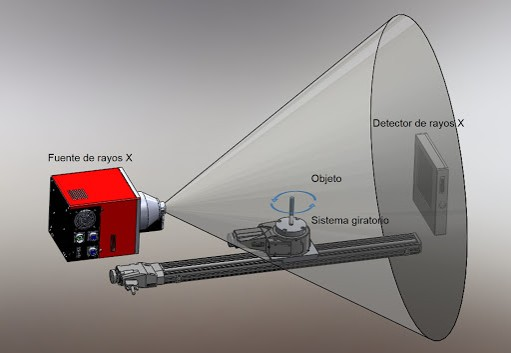
\includegraphics[width=0.5\textwidth]{images/esquema_microtomografo.jpg}
    \caption{Esquema de un sistema de microtomografía}
    \label{fig:esquema_tomografo}
\end{figure}

\section{Aparato Experimental: Microtomógrafo}

\subsection{Hardware}

Antes de entrar en detalle en el proceso de calibración, es esencial describir el
microtomógrafo sobre el que se realizó la totalidad de este trabajo. El mismo
forma parte del equipamiento del Laboratorio de Análisis de Materiales por 
Espectrometría de Rayos X (LAMARX), ubicado en la Facultad de Matemática, Astronomía,
Física y Computación de la Universidad Nacional de Córdoba (FAMAF-UNC). Se trata
de un equipo no comercial, ensamblado in situ, y cuenta con los siguientes
componentes:

\begin{enumerate}[label=\alph*)]
    \item Fuente de Rayos X: con un voltaje operacional en el rango 20-90 keV, una
    corriente de 10-200 $\mu$A (con un output máximo de 8 W). Posee un blanco de
    tungsteno y un tamaño de foco de 7 $\mu$m (5$\mu$m a 4 W); una ventana de berilio
    de 150 $\mu$m a una distancia de 9.5 mm del foco. El cono de rayos X emitido
    tiene un ángulo de apertura de 39$^{\circ}$ \cite{manual_fuente}.
    \item Detector Teledyne DALSA Shad-o-Box 6K HS, con centellador: con un área activa de $11.4\times
    14.6\text{ cm}^2$ (2304$\times$2940 pixeles), una resolución $\Delta p= 49.5\mu\text{m}$
    (tamaño de pixel) y un frame rate de 15 fps \cite{manual_detector}.
    \item Porta-muestra: Base de 5 cm de diámetro (intercambiable) con tres grados
    de libertad de movimiento. Movimiento longitudinal a través de un brazo mecánico
    controlado por un micro-motor, rango de $\sim 30$ cm y paso de 0.00635 mm. Movimiento
    vertical a través de un micro-motor, rango de $\sim 5$ cm y paso de 0.1 mm.
    Movimiento rotacional alrededor del eje vertical, a través de un micro-motor,
    rango de 360$^{\circ}$, con pasos de $\sim 0.026$$^{\circ}$. A su vez, el brazo mecánico posee una
    cámara apuntando directamente al porta-muestra, conectada a una computadora.
    \item Caja interna de protección radiológica: formada por paredes de plomo de 5 mm de espesor,
    con un tamaño de $85\times 38\times 48\text{ cm}^3$. Contiene la
    fuente, el porta-muestra y el detector, y sus paredes son desmontables para poder
    operar en su interior.
    \item Caja externa de protección radiológica: Caja con paredes reforzadas con láminas de plomo,
    con un tamaño de $150\times 120\times 100\text{ cm}^3$. Completamente cerrada, con dos
    puertas para acceder a su interior. Contiene todo el aparato en su interior sobre
    una mesa de mármol. Posee sensores en sus puertas que apagan la fuente al ser
    abiertas, si esta estaba en funcionamiento.
\end{enumerate}

En la figura \ref{fig:tomografo}.a se muestra la caja exterior, dentro de la cual está
contenido el microtomógrafo. En la figura \ref{fig:tomografo}.b puede observarse la
disposición del microtomógrafo
previa a este trabajo, donde cada componente está posicionado sobre la mesa de mármol,
independiente uno de otro.
Aunque esto permite una fácil manipulación de cada elemento
individual, presenta en realidad una gran desventaja: el sistema es muy propenso a
desalineaciones accidentales, lo que implicaría la necesidad de una re-calibración. Para evitar esta
situación, uno de los primeros cambios que se implementaron fue fijar la fuente y
el detector sobre una base rígida, diseñada a medida y formada por caños rectangulares
de acero (ver figura \ref{fig:tomografo}.c). Para ello, fue necesario realizar
una serie de operaciones para alinear correctamente ambos elementos, las cuales están
explicadas en detalle en la sección \ref{sec:calibracion_espacial}. De esta forma, la fuente
y el detector quedan siempre fijos en relación al otro, y se elimina una de las posibles
causas de desalineación. Aún así, el porta-muestra permanece independiente del
sistema fuente-detector. La imagen \ref{fig:tomografo}.d muestra la disposición final del
sistema, similar a la de la figura \ref{fig:tomografo}.c pero con el detector rotado 90$^{\circ}$ en
sentido anti-horario. Este cambio se debe a que la mayoría de las muestras que uno estudia
con un microtomógrafo suelen ser más alargadas en su eje principal de simetría (el que se
usa como rotación), por lo que así se aprovecha mejor el área activa del detector, y se
evita el tener que rotar las imágenes.

\begin{figure}[t]
    \centering
    % Primera fila
    \begin{overpic}[width=0.45\linewidth]{images/caja_ext.png}
        \put(2, 65){\colorbox{black!60}{\color{white}\bfseries\large (a)}}
    \end{overpic}\hspace{2ex}
    \begin{overpic}[width=0.45\linewidth]{images/tomografo_antes.jpg}
        \put(2, 65){\colorbox{black!60}{\color{white}\bfseries\large (b)}}
    \end{overpic}
    
    \vspace{2ex} % Espaciado entre filas
    
    % Segunda fila
    \begin{overpic}[width=0.45\linewidth]{images/tomografo_ahora.jpg}
        \put(2, 65){\colorbox{black!60}{\color{white}\bfseries\large (c)}}
    \end{overpic}\hspace{2ex}
    \begin{overpic}[width=0.45\linewidth]{images/sist_final.jpeg}
        \put(2, 65){\colorbox{black!60}{\color{white}\bfseries\large (d)}}
    \end{overpic}
    
    \caption{\textbf{a)} Caja de contención externa, equipada con alarma y apagado automático.
    \textbf{b)} Distribución original del micro-tomógrafo. Todos los elementos están separados
    y son independientes. \textbf{c)} Segunda iteración del micro-tomógrafo. Fuente y detector
    están fijos y alineados sobre una base de metálica. \textbf{d)} Última iteración del sistema.
    Se rotó 90$^{\circ}$ en sentido anti-horario el detector.}
    \label{fig:tomografo}
\end{figure}


Otro cambio realizado fue el diseño de una serie de porta-muestras cilíndricos con láminas
de plástico. Estos sirven para contener objetos suspendidos en algodón, material que es casi transparente
para los rayos X, pudiendo adquirir imágenes de las muestras sin que estas sean
opacadas por la base en la que se ubican.



\subsection{Software}

El software de adquisición de imágenes del microtomógrafo es \textit{Sapera LT} y \textit{CamExpert},
desarrollados ambos por la empresa Teledyne DALSA \cite{manual_detector}. Para controlar los
micro-motores del sistema, y para integrar las rutinas de adquisición, se utilizó un software de control
desarrollado en el laboratorio. Y para la reconstrucción de las tomografías, se utilizó el software
comercial \textit{NRecon} (utilizado por marcas comerciales de microtomógrafo como \textit{Bruker}),
que implementa el algoritmo de retroproyección filtrada
y permite realizar algunas correcciones geométricas previas.

Por otro lado, el principal software utilizado para el análisis y para el procesamiento de
proyecciones y tomografías fue \textit{FIJI-ImageJ} \cite{FIJI}\cite{FIJI2}. Este es un software gratuito
y de código abierto, con una amplia gama de herramientas para la investigación científica
a partir de imágenes digitales, con la capacidad de realizar análisis cuantitativos, operaciones
matemáticas complejas, transformaciones geométricas, segmentación, etc. Además, permite la
creación de \textit{macros} y \textit{plugins} personalizados (los cuales pueden ser compartidos con la comunidad),
lo que lo convierte en una herramienta muy versátil para este trabajo. Para la visualización de las tomografías, se utilizó el software gratuito \textit{3D Slicer} \cite{3DSlicer1}
\cite{3DSlicer2}, también de código abierto y con amplias posibilidades de análisis.

También se utilizó el software \textit{TASMIP} \cite{TASMIP}, para la simulación de espectros
de rayos X emitidos por la fuente, en función del voltaje aplicado, el material del blanco, y
cualquier posible filtro utilizado. Este software provee una simulación lejos de ser exacta,
pero que permite obtener una aproximación general de la distribución de energía del haz.

Por último, para el análisis y procesamiento de datos y resultados, se implementaron códigos
personalizados en Python.

\section{Desalineaciones del sistema}

Todos los componentes del sistema deben estar alineados sobre un mismo eje, denominado el \textit{eje
de magnificación}, o eje $\mathcal{M}$ (ver figura \ref{fig:sist_coord}.a). Este coincide con el eje
principal del cono de rayos X emitidos por la fuente y es normal al plano $\mathcal{D}$ de la
pantalla del detector. Para este trabajo, se definen los siguientes sistemas de
coordenadas. El sistema de coordenadas del mundo, con origen en el foco de la fuente, y ejes $X$, $Y$ y $Z$,
donde $X$ coincide con el eje $\mathcal{M}$, $Y$ es paralelo al plano $\mathcal{D}$ y $Z$
es perpendicular a ambos (hacia arriba). El sistema de coordenadas del detector, cuyos ejes $U$, $V$
son paralelos a la cuadrícula de pixeles del detector, y $W$ paralelo a $X$; y su origen se encuentra en su centro geométrico.
El sistema de coordenadas del porta-muestra, con origen en el eje rotación, el eje $\hat{Z}$, y ejes
$\hat{X}$ (definido por la dirección del brazo mecánico) e $\hat{Y}$ (perpendicular a ambos).
Por último, el sistema de coordenadas de la cuadrícula de pixeles (propia del detector) con ejes $u$ y $v$
ortogonales a $U$ y $V$, pero no con el mismo sentido ni origen.

Por defecto, el detector debería estar rotado 90$^{\circ}$ en dirección contraria a las agujas del
reloj respecto de lo que se observa en las
figuras \ref{fig:tomografo}.c y \ref{fig:sist_coord}, ya que el origen ``real'' (donde se comienza
a contar la posición de los pixeles) está en la esquina superior derecha (cuadrante $U>0$ y
$V>0$). La posición en la que se encuentra el detector, a pesar de ser ``incorrecta'' inicialmente, no
implica ningún problema para la adquisición, puesto que puede arreglarse fácilmente rotando
todas las imágenes obtenidas 90$^{\circ}$ en la dirección de las agujas del reloj (lo cual puede ser
automatizado mediante un \textit{macro} en FIJI). Esta rotación, al ser de 90$^{\circ}$, no necesita de ninguna
interpolación de pixeles, por lo que la imagen obtenida es esencialmente la misma que la
original. Pero esta transformación corre también el origen y los ejes de coordenadas $(u,v)$ de
la cuadrícula de pixeles, a la esquina superior izquierda ($U<0$ y $V>0$, ver figura
\ref{fig:sist_coord}). Como en todo este trabajo se utilizaron las imágenes rotadas, y no
las imágenes por defecto, se define el sistema de coordenadas $(u,v)$ como el que se observa en la
figura \ref{fig:sist_coord}.b, tal que su relación con los ejes $U$ y $V$ está dada por
$U = u_0 + u$ y $V = v_0 - v$, donde $(u_0,v_0)$ es el centro geométrico del detector en el
sistema $(u,v)$. Solamente para la última modificación del sistema (en la que se rotó el detector),
se utilizó como sistema $U = u - u'_0$ y $V = v'_0 - v$, donde $(u'_0,v'_0)$ es el nuevo centro geométrico
del detector (se sigue trabajando con $(u,v)$ como origen en la esquina superior izquierda de la imagen).

Por otro lado, es importante aclarar que a lo largo de este trabajo se han realizado numerosas
comparaciones entre mediciones en el mundo ``real'' y mediciones a partir de imágenes. Para
no dar lugar a ambigüedades, todas las mediciones de longitud (y por consiguiente área y volumen),
se asumirán con unidades de medida reales, es decir, del Sistema Internacional. Si una distancia $a$ se mide en una imagen,
entonces se tiene la siguiente relación: $a_{real} = M\cdot a_{proy} = M\cdot \Delta p
[\mu\text{m/px}] \cdot a_{img}[\text{px}]$,
donde $\Delta p$ es el ancho/altura de un pixel del detector. En adelante, toda distancia
medida a través de una imagen será entendida como $a_{proy}$ a menos que se especifique de
otra forma. Es decir, se entenderá como la distancia real proyectada sobre el plano $\mathcal{D}$
del detector, y no como una distancia en pixeles.

\begin{figure}[htpb]
    \centering
    \begin{subfigure}{0.58\textwidth}
        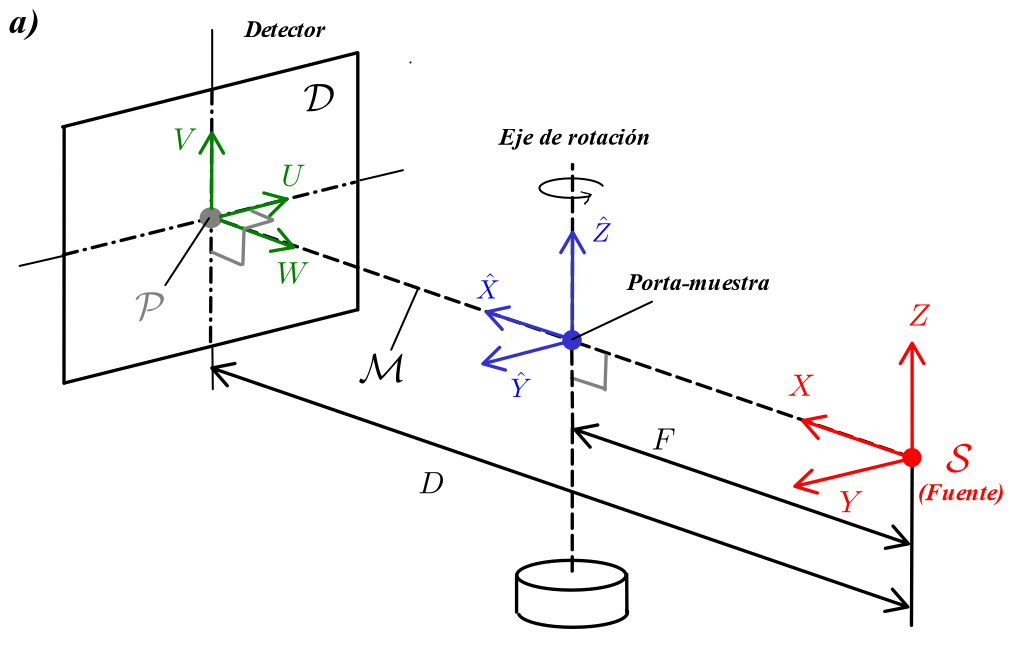
\includegraphics[width=\textwidth]{images/sist_coord1.png}
    \end{subfigure}
    \hfill
    \begin{subfigure}{0.40\textwidth}
        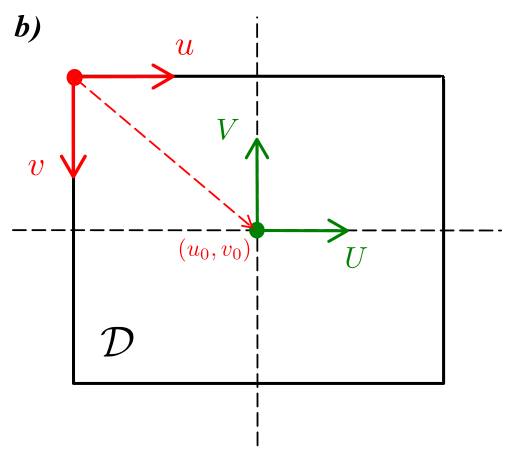
\includegraphics[width=\textwidth]{images/sist_coord2.png}
    \end{subfigure}
    \caption{Sistemas de coordenadas de un sistema de $\mu$CT. \textbf{a)} Representación
    ideal del sistema. El eje de magnificación $\mathcal{M}$ (eje principal del cono de rayos X)
    define los ejes $(X,Y,Z)$ del mundo, con origen en el foco de la fuente ($\mathcal{S}$);
    los ejes $\hat{X}$ del porta-muestra y $W$ del detector están alineados con $\mathcal{M}$;
    el eje $V$ del plano del detector ($\mathcal{D}$) es paralelo, en la misma dirección,
    que el eje de rotación de la muestra, $\hat{Z}$; el punto principal $\mathcal{P}$ se
    encuentra en el centro geométrico del detector; $\mathcal{P}$ y el porta-muestra están a
    distancias $D$ y $F$ del foco, respectivamente. \textbf{b)} Sistema de coordenadas propio
    de la imagen obtenida por el detector, $(u,v)$ y sistema de coordenadas $(U,V)$ empleado
    para la alineación, con origen en el centro geométrico $(u_0,v_0)$.}
    \label{fig:sist_coord}
\end{figure}

Para obtener una reconstrucción precisa a partir de las proyecciones, el algoritmo de
de retroproyección filtrada asume un sistema con una serie de características ideales.
Se define una desalineación como \textit{cualquier desviación geométrica del sistema
ideal que produce un artefacto}, también llamada comunmente en la literatura \textit{factor
de influencia}. Cada tipo de desalineación tiene un parámetro
geométrico $\zeta$ asociado, tal que $\zeta = 0$ corresponde a un estado ideal
del sistema. A continuación, se detallan las características de un sistema ideal,
así como sus posibles desalineaciones y parámetros geométricos correspondientes
\cite{Sun2006}\cite{Ferrucci2015}\cite{Yang2006}.

\begin{enumerate}[label=\alph*)]
    \item La intersección del eje $\mathcal{M}$ con el plano $\mathcal{D}$, llamado
    \textit{punto principal} $\mathcal{P}$ se encuentra en el centro geométrico
    del detector. El sistema está desalineado si $\mathcal{P}=(\Delta U, \Delta V)$.
    \item El eje $\mathcal{M}$ incide normalmente sobre el plano $\mathcal{D}$. El
    sistema está desalineado si existe alguna inclinación en las dos direcciones
    posibles, y los parámetros geométricos asociados son los ángulos $\theta$ y $\phi$
    (también llamados ángulos ``fuera de plano'').
    \item El eje $\hat{X}$ del porta-muestra coincide con el eje $\mathcal{M}$
    El sistema está desalineado si el eje $\hat{X}$ forma un ángulo $\psi$ con el 
    eje $\mathcal{M}$, o si está desplazado una distancia $\Delta \hat{Y}$ respecto
    de este.
    \item El eje $\hat{Z}$ de rotación del porta-muestra es paralelo al plano $\mathcal{D}$.
    El sistema está desalineado si el eje $\hat{Z}$ forma un ángulo $\vartheta$ con el plano
    $\mathcal{D}$.
    \item El eje $\hat{Z}$ es paralelo al eje $V$ del detector. El sistema está desalineado
    si el eje $\hat{Z}$ forma un ángulo $\eta$ con el eje $V$ (rotación del sistema $(U,V)$
    en el plano $\mathcal{D}$).
    \item El sistema tiene una magnificación $M$ definida por las distancias $D$
    (fuente-detector) y $F$ (fuente-objeto) como indica la ec. \ref{eq:magnificacion}.
    El sistema está desalineado si $M$ no es la esperada, es decir, si existen errores
    $\Delta D$ o $\Delta F$ en la determinación de estas distancias. 

\end{enumerate}

\section{Calibración espacial} \label{sec:calibracion_espacial}

Los parámetros geométricos del sistema son $\{\Delta U, \Delta V, \theta,
\phi, \psi, \Delta \hat{Y}, \vartheta, \eta, \Delta D, \Delta F\}$. El objetivo de la
calibración espacial es reducir o determinar cada uno de estos parámetros
para obtener proyecciones lo más fieles posibles a la realidad, de forma tal que las
mediciones espaciales (distancias, ángulos, etc.) sean lo más precisas posibles. Se
lleva a cabo en dos etapas: una alineación directa del sistema (hardware) por medio
de un ajuste físico de los componentes y una calibración fina, dada por la determinación de
los parámetros geométricos restantes, para una posterior corrección de las proyecciones
(software). Dispositivos comerciales como los de Bruker también tienen sus propios
métodos y software de calibración, a pesar de ya estar ensamblados y supuestamente bien
alineados, y en general estos están basados en principios que se detallan a continuación.

\subsection{Alineación del sistema}

Una primera alineación óptima del sistema reduce drásticamente la cantidad de correcciones
a realizar en el procesamiento de las proyecciones. Para ello, se diseñó y planificó el
siguiente procedimiento.

En primer lugar, se buscó alinear la fuente y el detector para fijarlos sobre la base
rígida, es decir, se trataron los casos a) y b) de la sección anterior. Inicialmente se utilizó
un nivel óptico y un nivel láser para buscar que los componentes sean lo más paralelos posible
a la superficie. Posteriormente, se
estudió la proyección del cono sobre el detector a una distancia cercana y lejana a la
fuente (sin ninguna muestra). La imagen proyectada es, esencialmente, la intersección de
un cono con el plano $\mathcal{D}$, luego esta toma la forma de un círculo si el plano
es perpendicular al eje principal del cono (el eje $\mathcal{M}$), o una elipse si 
existe alguna inclinación fuera de plano. Rotando muy de a poco el detector, 
se pueden reducir los ángulos $\theta$ y $\phi$. 
Por otro lado, para hacer coincidir el punto principal $\mathcal{P}$
con el centro del detector, se ajustó manualmente la posición de este con respecto a la
fuente hasta acercar ambos puntos lo máximo posible. Una vez se hicieron ambas cosas,
se alejó el detector a una distancia tal que el círculo proyectado ocupaba casi toda
la pantalla, y se repitió todo el procedimiento anterior. De esta forma, iterando varias
veces entre ambas posiciones del detector, es posible reducir los parámetros $\Delta U$,
$\Delta V$, $\theta$ y $\phi$ (ver figura \ref{fig:alineacion_fuente}). Para todo este
procedimiento, se diseñó un \textit{macro} en FIJI, capaz de binarizar la imagen, hallar los centros
de las figuras y calcular los criterios de similitud presentados en la ec. \ref{eq:circ_R},
para facilitar el trabajo y el análisis. El mismo está adjunto en el Apéndice B.1.

Es importante destacar que la posición final del detector es más alejada que cualquiera
de las posiciones utilizadas para la alineación, ya que el cono de rayos X debe llegar
a cubrir toda la pantalla. Es decir, una vez encontradas la dirección y orientación
correctas, a partir del método anterior, se aleja el detector una distancia adecuada,
con cuidado de mantenerlo en la misma línea imaginaria (eje $\mathcal{M}$). 

\begin{figure}[htpb]
    \centering
    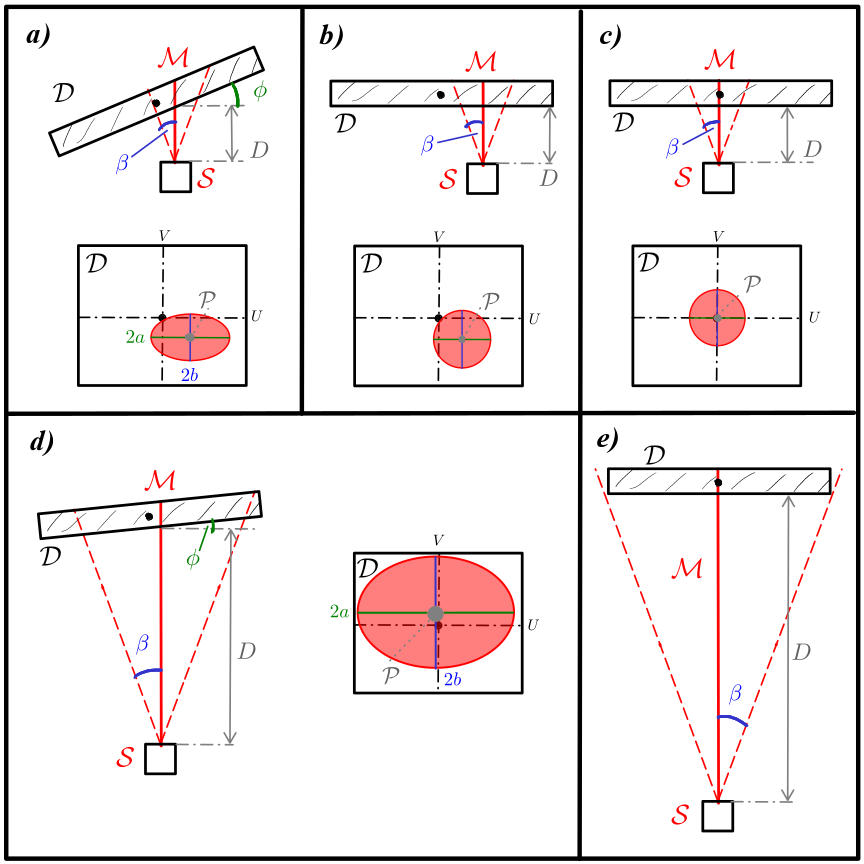
\includegraphics[width=\textwidth]{images/alineacion_fuente.png}
    \caption{Proceso de alineación fuente-detector (visto desde ``arriba''). \textbf{a)} Detector
    inicialmente desalineado, con inclinación y desplazamiento (en este caso, solo inclinación $\phi$
    alrededor de $V$, y desplazamiento en $Y$ y $Z$) con respecto a la fuente y al eje $\mathcal{M}$.
    La proyección del cono será una elipse desplazada del centro. \textbf{b)} Tras rotar correctamente
    el detector hasta colocarlo paralelo al eje $\mathcal{M}$, la elipse proyectada se convierte
    en un círculo. \textbf{c)} Manteniendo la orientación, se desplaza vertical y horizontalmente
    el detector, hasta lograr que el punto principal $\mathcal{P}$ coincida con el centro de la
    pantalla. \textbf{d)} Se aleja el detector a una distancia intermedia, y se repite el procedimiento
    anterior. Posteriormente, se verifica que en la primera distancia siga estando alineado. \textbf{e)}
    Una vez que el detector se encuentra alineado en todo el trayecto evaluado, se lo lleva a
    su posición final, lo suficientemente alejado como para que la proyección del cono apenas supere
    toda la pantalla.}
    \label{fig:alineacion_fuente}
\end{figure}

Una vez fijos la fuente y el detector, se procedió a alinear el porta-muestra, específicamente
los casos c) y e) de la sección anterior. Para esto, se colocó un objeto cilíndrico y alargado
en la dirección vertical, y se realizó un procedimiento similar al anterior (distancias cercana $x_1$
y lejana $x_2$ a la fuente). En cada posición, se tomaron dos proyecciones, una de ellas con 
el porta-muestra rotado 180$^{\circ}$ con respecto a la otra. Reflejando esta última imagen (en el eje
vertical) y superponiéndola a la primera, se puede estudiar la alineación del porta-muestra.
Si las imágenes se superponen perfectamente en el centro, el porta-muestra está sobre el eje
$\mathcal{M}$ (a esa distancia $x_i$ específica), de lo contrario se observa una superposición
parcial o nula de los cilindros. La alineación se realiza comparando esta misma situación en las
dos distancias. Si en las dos sucede que al superponer las imágenes los cilindros
están separados, quiere decir que en ninguna posición intermedia el eje $\hat{X}$ interseca con
el eje $\mathcal{M}$, por lo que debe desplazarse todo el sistema de forma paralela. Una vez
se observa que en alguna distancia ocurre una superposición de los cilindros, se sabe que en ese
punto (o alguno cercano) se da la coincidencia de los ejes. Queda entonces inclinar levemente
el eje $\hat{X}$, hasta que la coincidencia ocurra también en el otro extremo $x_j$.
Después de múltiples iteraciones de este proceso, revisando en ambas distancias, se puede reducir
cada vez más la distancia y el ángulo entre los ejes, hasta obtener que los cilindros se superponen
completamente en ambas distancias. Para ello, se diseñó un \textit{macro} en FIJI que automatiza el proceso
(ver Apéndice B.2).

En la figura \ref{fig:alineacion_muestra} se observa con mayor detalle el proceso, y cómo la
inclinación y distancia entre los ejes se relaciona con la posición de los cilindros en las
imágenes superpuestas (una normal y la otra reflejada). En particular, se puede conocer (o
al menos aproximar) la distancia $d$ a la que se encuentra el eje $\hat{X}$ del eje $\mathcal{M}$
($d$ un segmento perpendicular a $\mathcal{M}$), en alguno de los puntos $x_i$, estudiando la
separación entre los centros de los cilindros $\Delta x_i$ en la superposición de imágenes.
Conociendo el diámetro real del cilindro, $\mathsf{D}_{real}$, y midiendo el diámetro magnificado en la imagen,
$\mathsf{D}_{mag}$, se puede calcular la magnificación $M(x_i)$. Así, se tiene

\begin{equation}
    d_i = \frac{\Delta d_i}{2M} = \frac{\Delta d_i}{2} \frac{\mathsf{D}_{real}}{\mathsf{D}_{mag}}
    \label{eq:alineacion_muestra}
\end{equation}


\begin{figure}[htpb]
    
    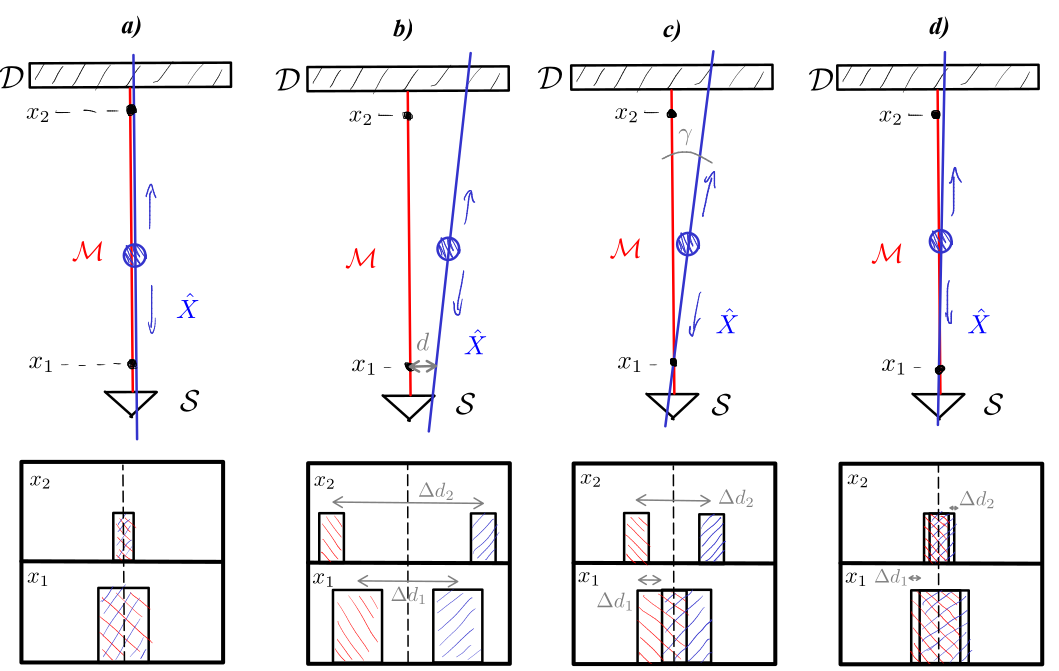
\includegraphics[width=\textwidth]{images/alineacion_muestra.png}
    \caption{Alineación del sistema fuente-detector (eje $\mathcal{M}$) con el eje de movimiento
    de la muestra (eje $\hat{X}$). Arriba se observa la posición de cada elemento del sistema, así
    como las distancias cercana y lejana a la fuente ($\mathcal{S}$), $x_1$ y $x_2$ respectivamente.
    Abajo se observan las imágenes superpuestas de los cilindros (rojo ``real'', y azul
    ``reflejada''), para cada distancia $x_i$. \textbf{a)} Estado ideal del sistema, con ambos
    ejes perfectamente alineados, y los cilindros completamente superpuestos en ambas distancias.
    \textbf{b)} Desalineación arbitraria del sistema, con el eje $\hat{X}$ desplazado e inclinado
    respecto a $\mathcal{M}$; en las dos distancias los cilindros se encuentran completamente
    separados. \textbf{c)} Intersección de los ejes en un punto cercano a $x_1$; superposición
    parcial de los cilindros en $x_1$. \textbf{d)} Reducción de la separación entre ejes; superposición casi
    completa de los cilindros, en ambas distancias.}
    \label{fig:alineacion_muestra}
\end{figure}

En realidad, aunque ambos ejes estén perfectamente alineados, puede suceder que los cilindros no
se superpongan perfectamente. Esto se debe al caso \textbf{e)} de las desalineaciones presentadas,
una inclinación $\eta$, en el plano $\mathcal{P}$, entre los ejes $V$ y $\hat{Z}$ (eje de rotación).
Este ángulo se puede aproximar a través de la misma superposición de los cilindros (real y reflejado).
Para ello, se trazan los ejes principales de cada cilindro, y se mide el ángulo entre ellos. Si
$\eta=0$, los ejes están perfectamente superpuestos y no hay ángulo. Si el cilindro está inclinado
hacia el eje $\hat{Y}$ a causa del porta-muestra, entonces su reflexión se verá inclinada hacia el
otro lado, el mismo ángulo. Por lo tanto, el ángulo medido entre los dos ejes proyectados es $2\eta$
(ver figura \ref{fig:alineacion_eta}).

\begin{figure}[htpb]
    \centering
    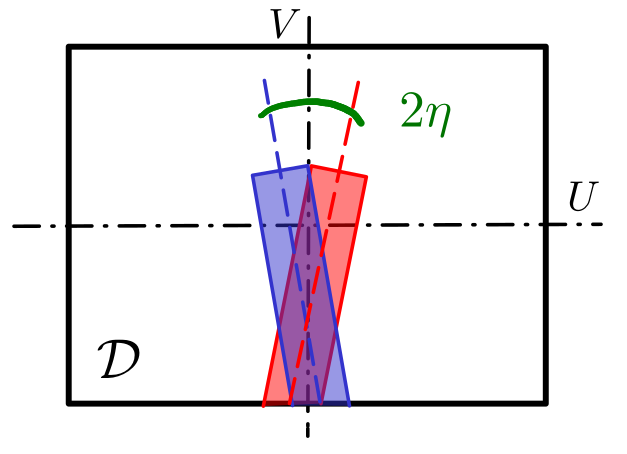
\includegraphics[width=0.4\textwidth]{images/alineacion_eta.png}
    \caption{Determinación de la inclinación $\eta$ (en el plano $\mathcal{D}$) a través de la
    superposición de la proyección de una muestra cilíndrica recta, y su reflexión tras rotarla
    180$^{\circ}$.}
    \label{fig:alineacion_eta}
\end{figure}

Hasta ahora, estos métodos requieren de una constante intervención y manipulación del hardware: movimiento,
inclinación y ajuste de todas las piezas involucradas. Y aunque las mejoras obtenidas en la reconstrucción
pueden ser drásticas, son limitadas por la destreza del operario y los instrumentos que tenga a su
disposición. A continuación, se mostrará un método de determinación de parámetros de forma analítica.

\subsubsection{Determinación de correcciones finas}

Existen numerosos métodos basados en la derivación analítica de las expresiones matemáticas
que relacionan mediciones obtenidas con los distintos factores de influencia, bajo un marco
o modelo de medición (en este caso, de un sistema de haz cónico) \cite{Ferrucci2015}.
Muchos de estos utilizan objetos de referencia (comúnmente llamados \textit{fantomas}), cuya
geometría es bien conocida, para extraer información de las proyecciones. En particular, muchos
de los métodos existentes para determinar los parámetros geométricos mencionados
utilizan fantomas que contienen esferas pequeñas y de alta densidad (o alta atenuación), que
funcionan como \textit{puntos marcadores} de coordenadas en las imágenes proyectadas, para obtener
mediciones precisas. A continuación se detallan dos métodos en particular, uno basado en una rotación
ideal del porta-muestra (es decir, requiere proyecciones de múltiples ángulos), y otro basado en
una posición fija del porta-muestra.

\medskip
\textit{A.Método de múltiples proyecciones.}
\smallskip

Si se considera un sistema cuyo porta-muestra rota de forma ideal (el eje $\hat{Z}$ permanece siempre
fijo), entonces un punto marcador ubicado fuera del eje de rotación recorrerá una trayectoria
circular. En un sistema de haz cónico, dicha trayectoria se proyecta sobre el plano del detector
como una elipse o una línea recta (en el caso específico en que la esfera gira sobre un plano que
contenga el eje $\mathcal{M}$). Aprovechando este hecho, se han diseñado múltiples fantomas
alrededor del mismo principio: el análisis geométrico de elipses proyectadas en el detector,
a partir de varios puntos marcadores (esferas pequeñas o ``ball bearings'' - BB's) rotando. \cite{Ferrucci2015} \cite{Noo2000}.
El método detallado a continuación fue desarrollado por Yang \textit{et al.} \cite{Yang2006}, y sirve
para determinar los parámetros {$\Delta U, \Delta V, \eta, D, F$}, mediante técnicas de regresión
lineal.

Para este análisis, se asume que las inclinaciones fuera del plano $\mathcal{D}$ ($\theta$ y
$\phi$) son despreciables, es decir, menores a 5$^{\circ}$. Esto es posible gracias a la observación
experimental de von Smekal \textit{et al.} \cite{Smekal2004} y su posterior demostración analítica por
Yang \textit{et al.} \cite{Yang2006}. Esto es, las distorsiones en la imagen provocadas por estas desviaciones
son mínimas; en concreto, para un haz cónico con semi-ángulo de apertura $\beta=20$$^{\circ}$, el error
porcentual en la posición proyectada de un punto marcador es menor al $4\%$ (y este valor es
alcanzado solo en los bordes de la pantalla, lejos del centro del cono), como se observa en los gráficos
de la figura \ref{fig:graf_yang1}.

\begin{figure}[htpb]
    \centering
    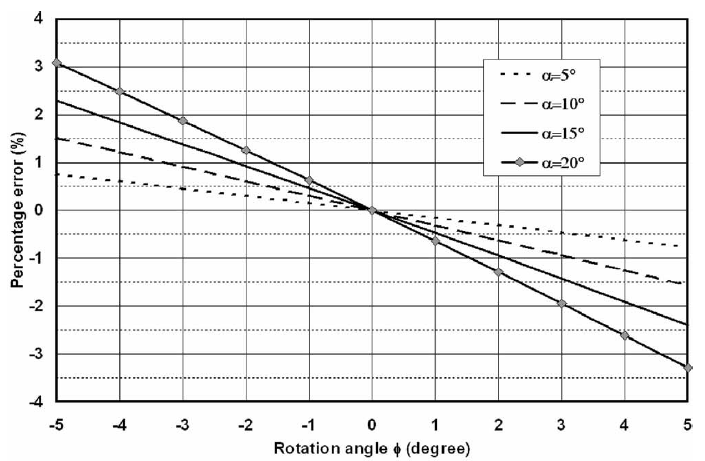
\includegraphics[width=0.65\textwidth]{images/graf_yang1.png}
    \caption{Error relativo de la posición proyectada de un punto marcador (respecto a la posición
    ideal) en función del ángulo fuera de plano $\phi$ (el caso es análogo para $\theta$), para un haz cónico de
    apertura $2\alpha$ ($2\beta$ en este trabajo). Gráfico extraído de Yang \textit{et al.} \cite{Yang2006}.}
    \label{fig:graf_yang1}
\end{figure}

Como fantoma, se utiliza un cilindro vertical de algún material de baja atenuación, con una serie
de esferas metálicas como puntos marcadores, alineadas verticalmente en la superficie del cilindro
(ver figura \ref{fig:metodo_yang}.a).
No es estrictamente necesario que sean equidistantes, pero resulta conveniente. Para cada marcador
$i$, se identifican en su trayectoria elíptica cinco puntos de referencia $\vec{p}_{ij} = (u_{ij},v_{ij})$
($0 \leq j\leq 4$). $j=0$ corresponde al centro geométrico de la elipse, mientras que $j=1,2,3,4$ 
están determinados a partir de las distancias máximas y mínimas entre "pares radiales" (puntos
desfasados 180$^{\circ}$ en la rotación), que coinciden con los cuatro vértices de la elipse proyectada
(ver figura \ref{fig:metodo_yang}.b).
A partir de las coordenadas obtenidas, se definen las siguientes variables:

\begin{equation}
    \left\{
    \begin{aligned}
        x_i &= sgn(v_{i0} - v_0)\frac{v_{i3} - v_{i1}}{|\vec{p}_{i2} - \vec{p}_{i4}|}\\
        y_i &= \frac{v_{i3} + v_{i1}}{2}    
    \end{aligned}
    \right.
    \hspace{15mm}
    sgn(x)=
    \left\{
    \begin{aligned}
        -1 \hspace{5mm}& x<0\\
        1 \hspace{5mm}& x \geqslant 0
    \end{aligned}
    \right.
    \label{eq:variables_yang1}
\end{equation}

Como se demuestra en Yang \textit{et al.} \cite{Yang2006}, se puede ajustar los pares $(x_i,y_i)$ a
una función lineal $y = \mathsf{a_1} + \mathsf{b_1}\cdot x$, tal que 

\begin{equation}
    D = \mathsf{a_1} \hspace{15mm} (v_0 + \Delta V) = \mathsf{b_1}
    \label{eq:Delta_V_D}
\end{equation}

Donde $(u_0, v_0)$ es el centro
geométrico del detector. La razón de utilizar la función $sgn(v_{i0}-v_0)$ en la definición
de $x_i$ se debe a la interpretación de esta misma. $x_i$ es una cantidad cuyo módulo es lineal con
la longitud del eje menor de la elipse. $x_i$ comienza siendo negativo, para elipses ubicadas cerca de
$v=0$, y crece a medida que se acercan al centro; si la elipse está justo en el centro,
$x_i=0$, y a medida que se aleja nuevamente del centro, $x_i$ crece con valores positivos,
manteniendo así la linealidad con $y_i$ para todas las elipses. En realidad, el que define
el cambio de signo no es el centro geométrico, sino el punto principal $(u_0 +\Delta U,
v_0 + \Delta V)$, sin embargo, al ser $\Delta V$ uno de los valores que se desea determinar
con este cambio de variables, se asume que la distancia entre $\mathcal{P}$ y el centro
es lo suficientemente pequeña como para que el ajuste tenga sentido.

Por otro lado, conociendo las coordenadas de los centros de cada elipse, y el valor de
$\Delta V$, puede determinarse los parámetros $\Delta u$ y $\eta$, a partir del siguiente
ajuste lineal $u_{i0} = \mathsf{a_2} + \mathsf{b_2}\cdot v_{i0}$. De esta forma, se obtiene

\begin{equation}
    u_0 + \Delta U = \mathsf{a_2} + \mathsf{b_2}\cdot (v_0 + \Delta V)
    \hspace{15mm}
    \eta = \arctan(\mathsf{b_2})
    \label{eq:delta_u_eta}
\end{equation}

Finalmente, para determinar $F$ se requiere conocer la distancia real $l$ entre dos esferas,
$i=1,2$ (no necesariamente consecutivas), y medir la proyección análoga.

\begin{equation}
    F = \dfrac{l\cdot D}{\sqrt{ (\vec{p}_{10}-\vec{p}_{20})^2 + \left(\frac{\vec{p}_{12} - \vec{p}_{14}}{2}\right)^2
    + \left(\dfrac{\vec{p}_{22} - \vec{p}_{24}}{2}\right)^2 - \dfrac{(\vec{p}_{12} - \vec{p}_{14})(\vec{p}_{22} - \vec{p}_{24})}{2} }}
    \label{eq:F}
\end{equation}

La precisión de este método radica enteramente en la determinación de los puntos $\vec{p}_{ij}$
de cada elipse. Para ello, se comienza obteniendo $N$ proyecciones del cilindro en rotación
(en este trabajo siempre se utilizó $N=352$, aproximadamente una imagen cada desplazamiento
angular de 1$^{\circ}$). Se diseñó un \textit{macro} en FIJI (ver Apéndice B.3) con la tarea de binarizar cada imagen y obtener
las coordenadas de los centros de las esferas metálicas, proyectadas como círculos. A partir
de las $N$ posiciones de cada esfera, $(u_i^{(k)}, v_i^{(k)})$, se determinaron los parámetros
{$A, B, C, u_{i0}, v_{i0}$} de las elipses (ver ec. \ref{eq:elipse}), a través de un ajuste
lineal por cuadrados mínimos detallado por Noo \textit{et al.} \cite{Noo2000}. Diagonalizando la matriz
$\mathbb{A}$ de cada elipse, se calculan los semiejes $a$ y $b$, y se obtienen sus respectivos
autovectores $\mathbf{v_a}$ y $\mathbf{v_b}$. Luego, sabiendo que los puntos $\vec{p}_{ij}$
($j=1,...,4$) son vértices de la elipse, se tiene

\begin{equation}
    \begin{aligned}
        \vec{p}_{i1} &= \vec{p}_{i0} - b_i\cdot \mathbf{v}_{i,b}\\
        \vec{p}_{i2} &= \vec{p}_{i0} - a_i\cdot \mathbf{v}_{i,a}
    \end{aligned}
    \hspace{15mm}
    \begin{aligned}
        \vec{p}_{i3} &= \vec{p}_{i0} + b_i\cdot \mathbf{v}_{i,b}\\
        \vec{p}_{i4} &= \vec{p}_{i0} + a_i\cdot \mathbf{v}_{i,a}
    \end{aligned}
    \label{eq:vertices}
\end{equation}

\begin{figure}[htpb]
    \centering
    \begin{subfigure}{0.28\textwidth}
        \begin{overpic}
            [width=\textwidth]{images/fantom_yang_1.jpg}
            \put(3,85){\colorbox{black!60}{\color{white}\bfseries\large (a)}}
        \end{overpic}        
    \end{subfigure}
    \hfill
    \begin{subfigure}{0.28\textwidth}
        \begin{overpic}
            [width=\textwidth]{images/fantom_yang.jpg}
            \put(3,85){\colorbox{black!60}{\color{white}\bfseries\large (b)}}
        \end{overpic}        
    \end{subfigure}
    \hfill
    \begin{subfigure}{0.42\textwidth}
        \begin{overpic}
            [width=\textwidth]{images/vertices_elipse.png}
            \put(2,60){\colorbox{black!60}{\color{white}\bfseries\large (c)}}
        \end{overpic}        
    \end{subfigure}
    \caption{\textbf{a)} Fantoma utilizado en el método de Yang \textit{et al.} \cite{Yang2006}, con 8
    esferas metálicas como puntos marcadores. \textbf{b)} Fantoma ubicado sobre
    el porta-muestra. \textbf{c)} Proyección de la trayectoria de un punto
    marcador tras una rotación completa; se ajusta una elipse y a partir de los
    parámetros $A$, $B$, $C$, $u_0$ y $v_0$, se determinan los puntos de interés
    $\vec{p}_{ij}$, $j=0,1,2,3,4$.}
    \label{fig:metodo_yang}
\end{figure}

\medskip
\textit{B. Estimación de los ángulos $\theta$ y $\phi$.}
\smallskip

La determinación de los ángulos fuera del plano $\mathcal{D}$ es más complicada y requiere
de métodos más complejos, como análisis de Fourier \cite{Smekal2004} o simulaciones y
optimización numérica \cite{Johnston2008}. Sin embargo, para este trabajo bastará demostrar
que estos son despreciables (<5$^{\circ}$), para que el método de Yang \textit{et al.} \cite{Yang2006} sea aplicable.
Para ello, se propone lo siguiente, teniendo en cuenta el mismo principio que se utilizó en la alineación del sistema 
fuente-detector (ver figura \ref{fig:alineacion_fuente}).

La proyección del cono sobre el detector es una elipse cuando $\theta \neq 0$ o $\phi \neq 0$,
o más en general, cuando el plano $\mathcal{D}$ esté inclinado un ángulo $\alpha$ con respecto
al plano ideal, en cualquier dirección. Conociendo el semi-ángulo $\beta$ de apertura del cono,
y los ejes $a$ y $b$ de la elipse proyectada, es posible determinar $\alpha$ a partir de la
ecuación \ref{eq:alfa_proyeccion}. Utilizando un \textit{macro} en FIJI (Apéndice B.1), se binariza la imagen de
la elipse, y se ajusta sus semi-ejes, para luego determinar $\alpha$. Como $\alpha$ es una
composición de las rotaciones $\theta$ y $\phi$, estos no pueden ser mayores.

Este método es una estimación, ya que se realiza con imágenes en una posición anterior a
la definitiva. El detector, en su estado final, debe estar lo suficientemente alejado de
la fuente como para que el cono ilumine toda la pantalla, siendo imposible verificar su
proyección elíptica. En vez de eso, se mide la elipse de un estado anterior, en la etapa
final de la alineación, y se asume que el desplazamiento hacia la última posición mantiene
la orientación conseguida (lo cual, si no es un sistema mecanizado, depende enteramente
de la destreza del operario). Pero además de aproximar, podría utilizarse el valor de
$\alpha$ y la dirección en la que se inclina (rota alrededor del eje menor), para corregir
las imágenes.

\medskip
\textit{C. Método de única proyección.}
\smallskip

El método propuesto por Sun \textit{et al.} \cite{Sun2006} ofrece una alternativa analítica para la 
calibración geométrica de un sistema de $\mu$CT de haz cónico, con la ventaja distintiva de que
requiere únicamente una proyección de un fantoma de referencia en lugar de múltiples adquisiciones
a diferentes ángulos. Este método utiliza un fantoma de cuatro puntos marcadores (esferas metálicas)
dispuestos en los vértices de un cuadrado de lado $l$ conocido ($l=(35.0 \pm 0.5)$ mm). El objetivo es determinar los siete
parámetros principales de desalineación: $\Delta U$, $\Delta V$, $\eta$, $\theta$, $\phi$, $D$ y $F$.

Los autores llegan a expresiones analíticas que vinculan los parámetros, estudiando todas las
posibles transformaciones geométricas (ver ec. \ref{eq:coord_homog}) de la proyección del cuadrado,
cambiando un factor de influencia a la vez, partiendo de la configuración ideal, y llegando a un
estado de desalineación arbitraria del sistema. Esto es posible, nuevamente, gracias a que la
matriz de transformación $\mathbb{H}$ puede ser obtenida a partir de un producto de transformaciones
$\mathbb{H}_i$ más simples y en un orden específico. Así, los autores demuestran que las
proporciones de los lados del cuadrilátero proyectado en el detector dependen exclusivamente de los
ángulos de rotación y no de los desplazamientos.

El desarrollo matemático es complejo y extenso, por lo que se detalla en el Apéndice A. Sin embargo,
basta con saber que se deben medir las longitudes de los lados del cuadrilátero proyectado ($L_{12}$,
$L_{34}$, $L_{13}$, $L_{24}$), y conocer la longitud real $l$ del lado (ver figura \ref{fig:yisun}).
A partir de las proporciones $L_{12}/L_{34}$ y $L_{13}/L_{24}$, se pueden determinar los ángulos $\theta$
y $\phi$; con estos valores se puede obtener una corrección $\Delta x$ (relacionada con las distancias
$D$ y $F$); y finalmente, analizando la posición de uno de los vértices del cuadrilátero, y con los
valores anteriores, se pueden determinar $\Delta U$, $\Delta V$ y $\eta$.

Este método, además de requerir las mismas condiciones explicadas en los anteriores, asume algunas otras
características. En primer lugar, que el eje $\mathcal{M}$ pasa justo por el centro del cuadrado. Para
ello, se agregó otra esfera metálica también en el centro como ayuda para verificar esto. En segundo
lugar, se asume que el mismo eje de magnificación es perpendicular al plano del cuadrado. Para obtener esto, primero se
lo alineó rotado 90$^{\circ}$ (de perfil), donde es más fácil determinar la orientación correcta estudiando la superposición
de las esferas y del marco de acrílico, y luego se lo rotó 90$^{\circ}$. Posteriormente, se obtuvieron 20 proyecciones
distintas en un rango de 2$^{\circ}$ alrededor de este punto inicial, para determinar la más apropiada.

\begin{figure}[htpb]
    \centering
    \begin{subfigure}{0.45\textwidth}
        \begin{overpic}
            [width=\textwidth]{images/phantom_sun.png}
            \put(3,93){\colorbox{black!60}{\color{white}\bfseries\large (a)}}
        \end{overpic}
    \end{subfigure}
    \hfill
    \begin{subfigure}{0.48\textwidth}
        \begin{overpic}
            [width=\textwidth]{images/cuadrilatero.png}
            \put(3,93){\colorbox{black!60}{\color{white}\bfseries\large (b)}}
        \end{overpic}
    \end{subfigure}
    \caption{\textbf{a)} Fantoma utilizado a partir del método propuesto en Sun \textit{et al.} \cite{Sun2006}.
    \textbf{b)} Cuadrilátero proyectado en el detector para una desalineación arbitraria del sistema. A
    partir de las longitudes de los lados proyectados, las proporciones entre ellos y la longitud real,
    es posible determinar los parámetros geométricos del sistema.}
    \label{fig:yisun}
\end{figure}

\subsection{Resultados}

Se comenzó alineando la fuente y el detector como se indicó anteriormente (ver figura \ref{fig:alineacion_fuente}). La distancia
cercana entre la superficie del detector y el foco de la fuente es $D_1 = (63 \pm 1)$ mm,
y la lejana $D_2 = (133 \pm 1)$ mm (ambas medidas desde el foco hacia la pantalla, con un
medidor láser). Después de múltiples mediciones entre ambas distancias,
realizando pequeños ajustes a la posición horizontal, vertical y orientación de la fuente,
se obtuvieron las proyecciones de la figura \ref{fig:res_alin_fuente} (tras ser umbralizadas).
Utilizando un \textit{macro} (Apéndice B.1),
se ajustaron elipses, y se obtuvieron los parámetros $a$, $b$, $C_W$ y $R$, y se estimaron
los valores de $\Delta U$, $\Delta V$ y $\alpha$ en cada posición. Los valores resultantes
son los mínimos que se pudieron lograr en esta etapa, y posteriormente se trasladó el detector
a su posición final $D = (258 \pm 1)$ mm de la fuente, de tal forma que el cono cubriera toda
la pantalla.

\begin{figure}[htbp]
    \centering
    \begin{subfigure}{0.48\textwidth}
        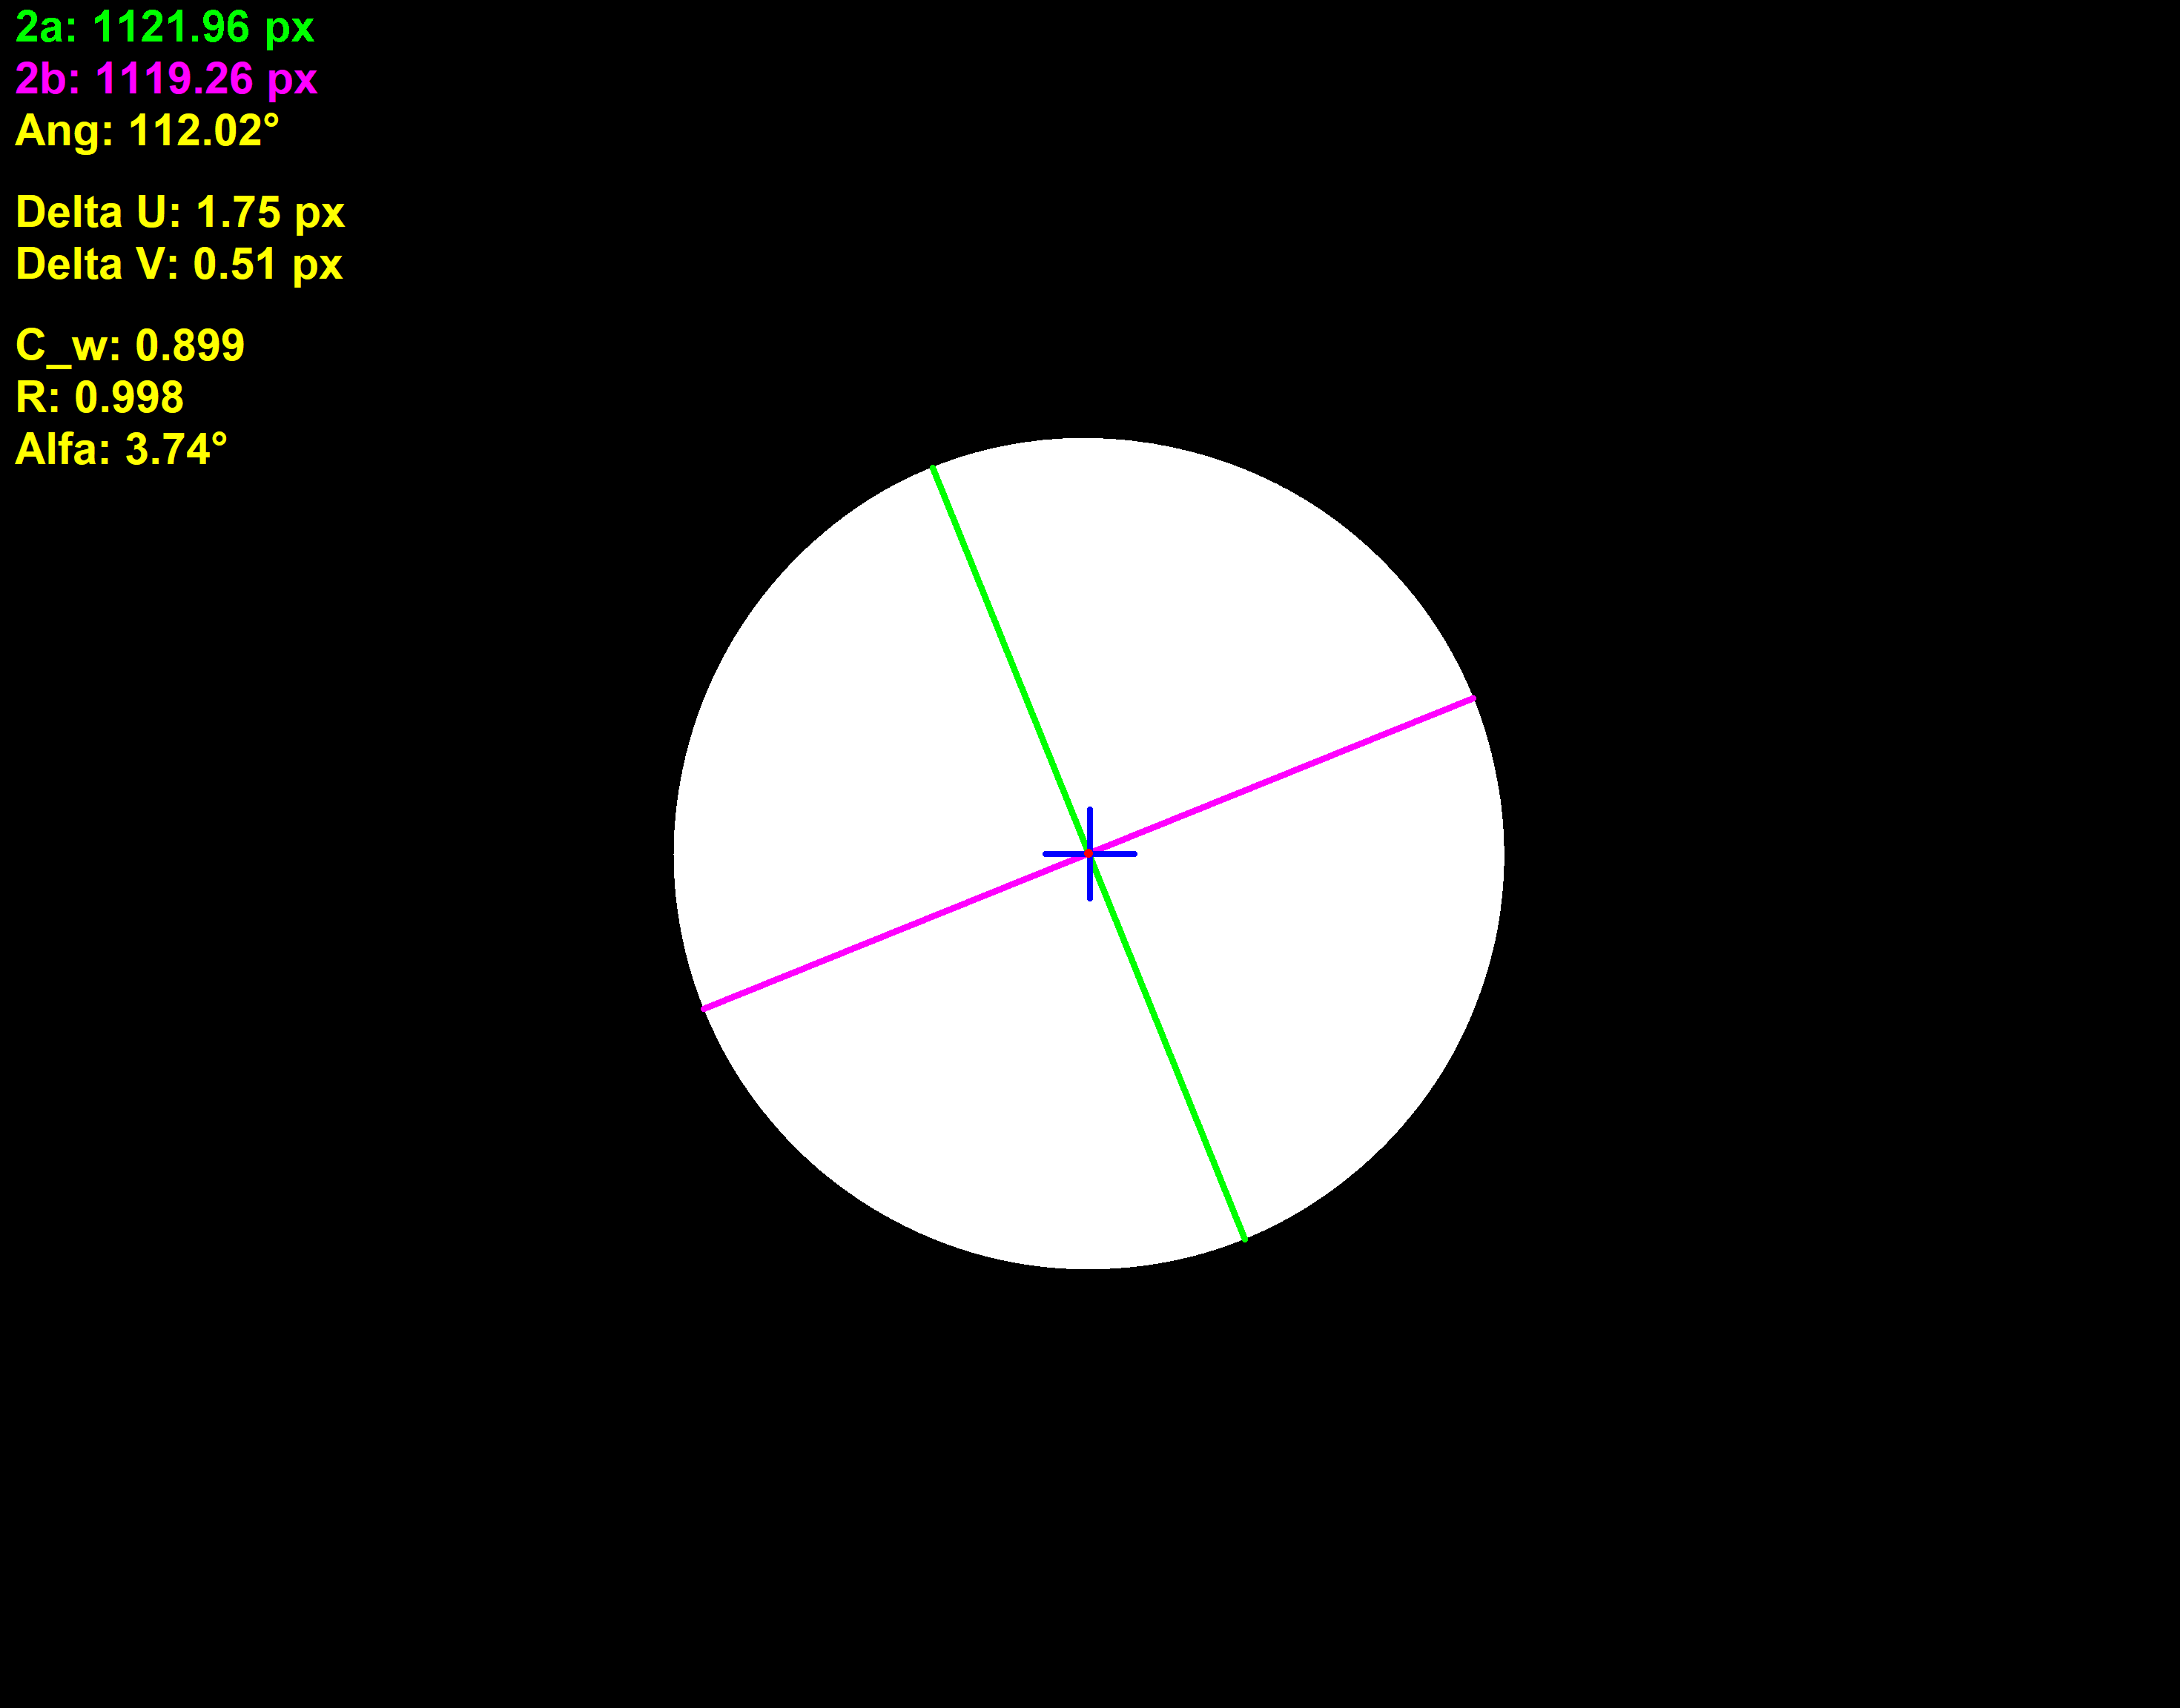
\includegraphics[width=\textwidth]{images/alineacion_cerca.png}
    \end{subfigure}
    \hfill
    \begin{subfigure}{0.48\textwidth}
        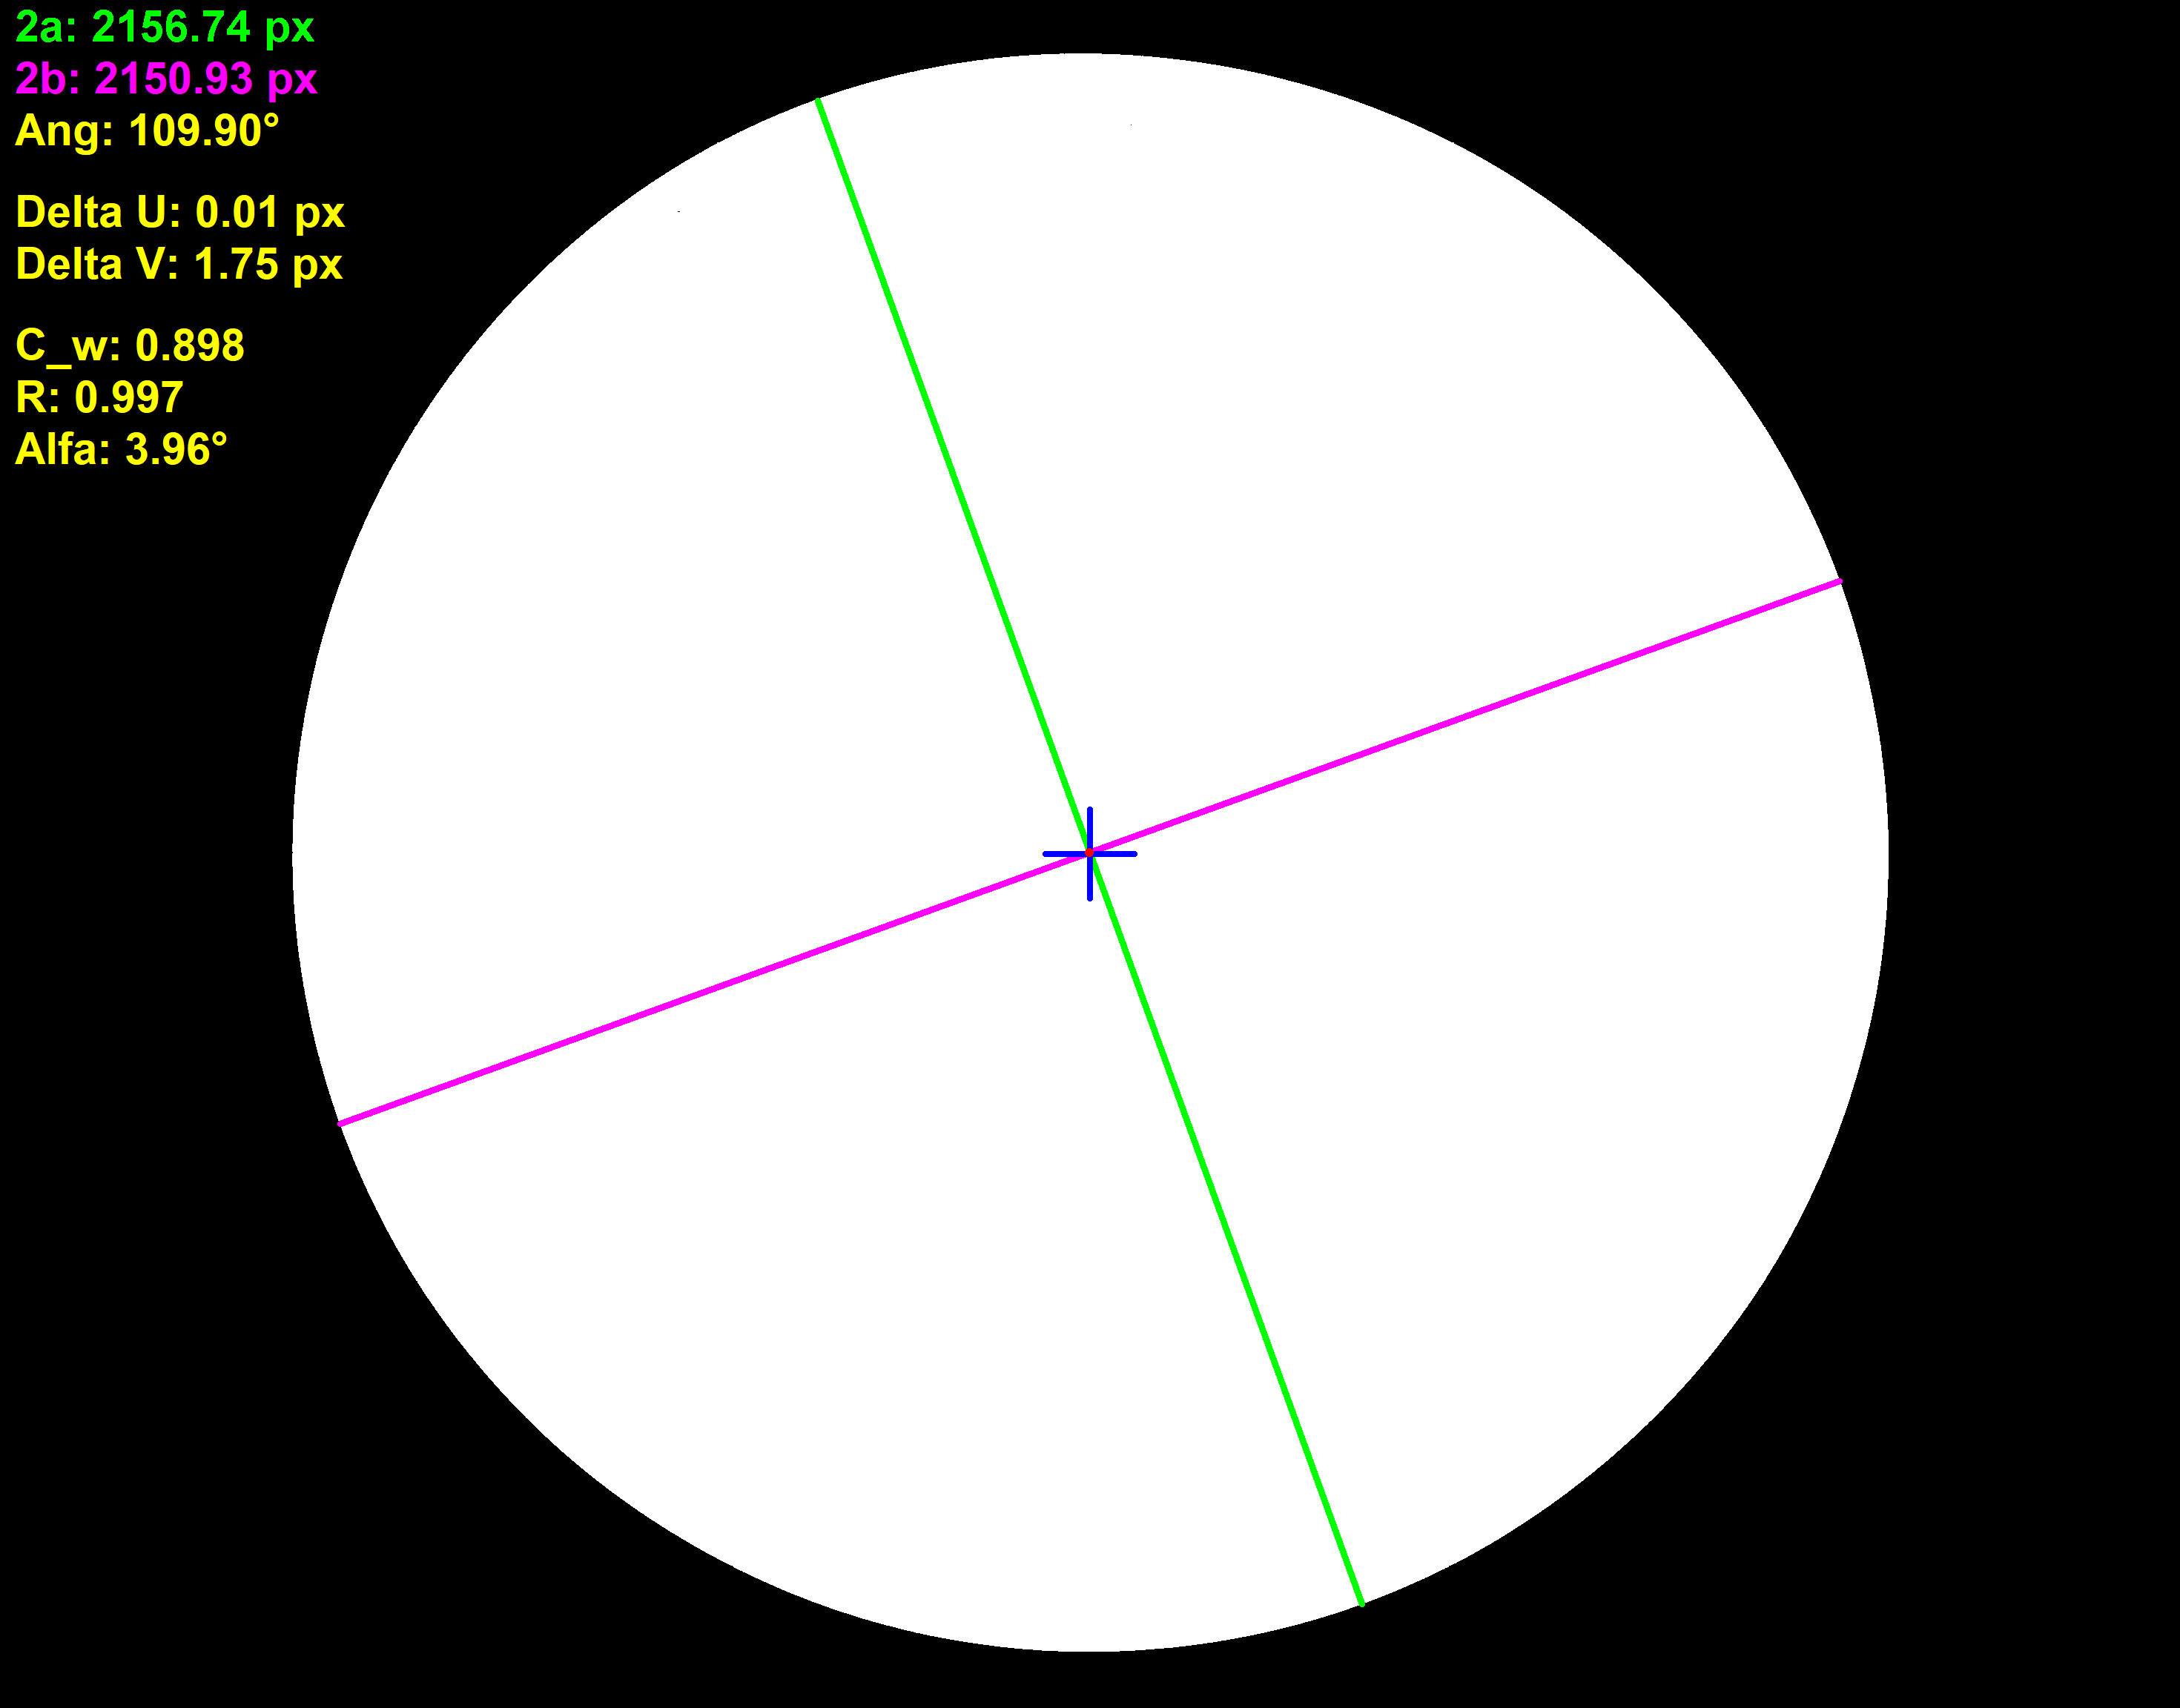
\includegraphics[width=\textwidth]{images/alineacion_lejos.png}
    \end{subfigure}
    \caption{Proyección del cono de rayos X sobre el detector a una distancia $D_1$ cercana
    (\textit{Izq.}) y $D_2$ lejana (\textit{Der.}). Las imágenes están umbralizadas para mostrar
    con mayor claridad, y para poder ajustar las elipses correspondientes, y así, obtener los
    parámetros $a$, $b$, Ang (dirección del eje mayor) $\Delta U$, $\Delta V$, $C_W$, $R$ y $\alpha$.}
    \label{fig:res_alin_fuente}
\end{figure}

Comparando los valores de $\Delta U$ y $\Delta V$ en cada posición, se puede estimar el ángulo $\varPhi$
entre el eje $\mathcal{M}$ y la dirección sobre la que se desplazó el detector a su posición
final. Como dicho desplazamiento se realizó ``a mano'', este ángulo no es una medición precisa,
sino más bien una forma de acotar $\Delta U$ y $\Delta V$ en la posición final (puesto
que no pueden ser medidos como en las posiciones anteriores). Así, se tiene que $\tan(\varPhi_U) \simeq
|\Delta U_1 - \Delta U_2| / |D_1 - D_2|$ y $\tan(\varPhi_V) \simeq |\Delta V_1 - \Delta V_2| / |D_1 - D_2|$,
y se obtiene que estos ángulos son menores a 0.1$^{\circ}$. Por lo tanto, en la posición final $D = (258 \pm 1)$ mm
se espera que $\Delta U, \Delta V < 5$ px. Por otro lado, la desviación del plano $\mathcal{D}$
con respecto al ideal es, en ambas posiciones, menor a 4$^{\circ}$; de la misma manera, se considera
que para la posición final, $\alpha < 4$$^{\circ}$ (cumpliéndose la condición para aplicar el método de múltiples proyecciones).

Fijados fuente y detector, se procedió a alinear el eje de movimiento del porta muestra, como
se indicó anteriormente. Se desplazó el objeto entre dos posiciones, separadas una distancia
$\Delta \hat{x} = (127 \pm 1)$ mm (sistema de coordenadas del eje de rotación). Las imágenes
superpuestas de objeto y su reflejo tras rotar
180$^{\circ}$ en cada posición, se pueden observar en la figura \ref{fig:res_alin_muestra}. Estas fueron
las últimas que se tomaron, tras repetir el proceso numerosas veces y realizar los ajustes
necesarios (como se explicó en la fig. \ref{fig:alineacion_muestra}). Las imágenes fueron umbralizadas
y coloreadas (verde para el objeto en 0$^{\circ}$ y rojo para el objeto en 180$^{\circ}$, y reflejado), para facilitar
el análisis. Con un \textit{macro} (Apéndice B.2), se superpusieron ambas imágenes (el color amarillo representa la región
de superposición entre los dos objetos), y se determinaron los ejes principales de cada objeto, el ángulo $2\eta$
entre ambos, y la distancia $\Delta d$ entre los ejes (medida sobre el eje $U$, es decir, $V=0$). Así, se tiene
que el desplazamiento del eje de rotación respecto al eje $\mathcal{M}$ es $\Delta \hat{y} <
2$ mm (alcanzando este valor solamente muy cerca de la fuente). Por otro lado, se estima que
la inclinación del eje respecto al eje $V$ del detector es $\eta = (0.48 \pm 0.06)$$^{\circ}$.

\begin{figure}[htbp]
    \centering
    \begin{subfigure}{0.49\textwidth}
        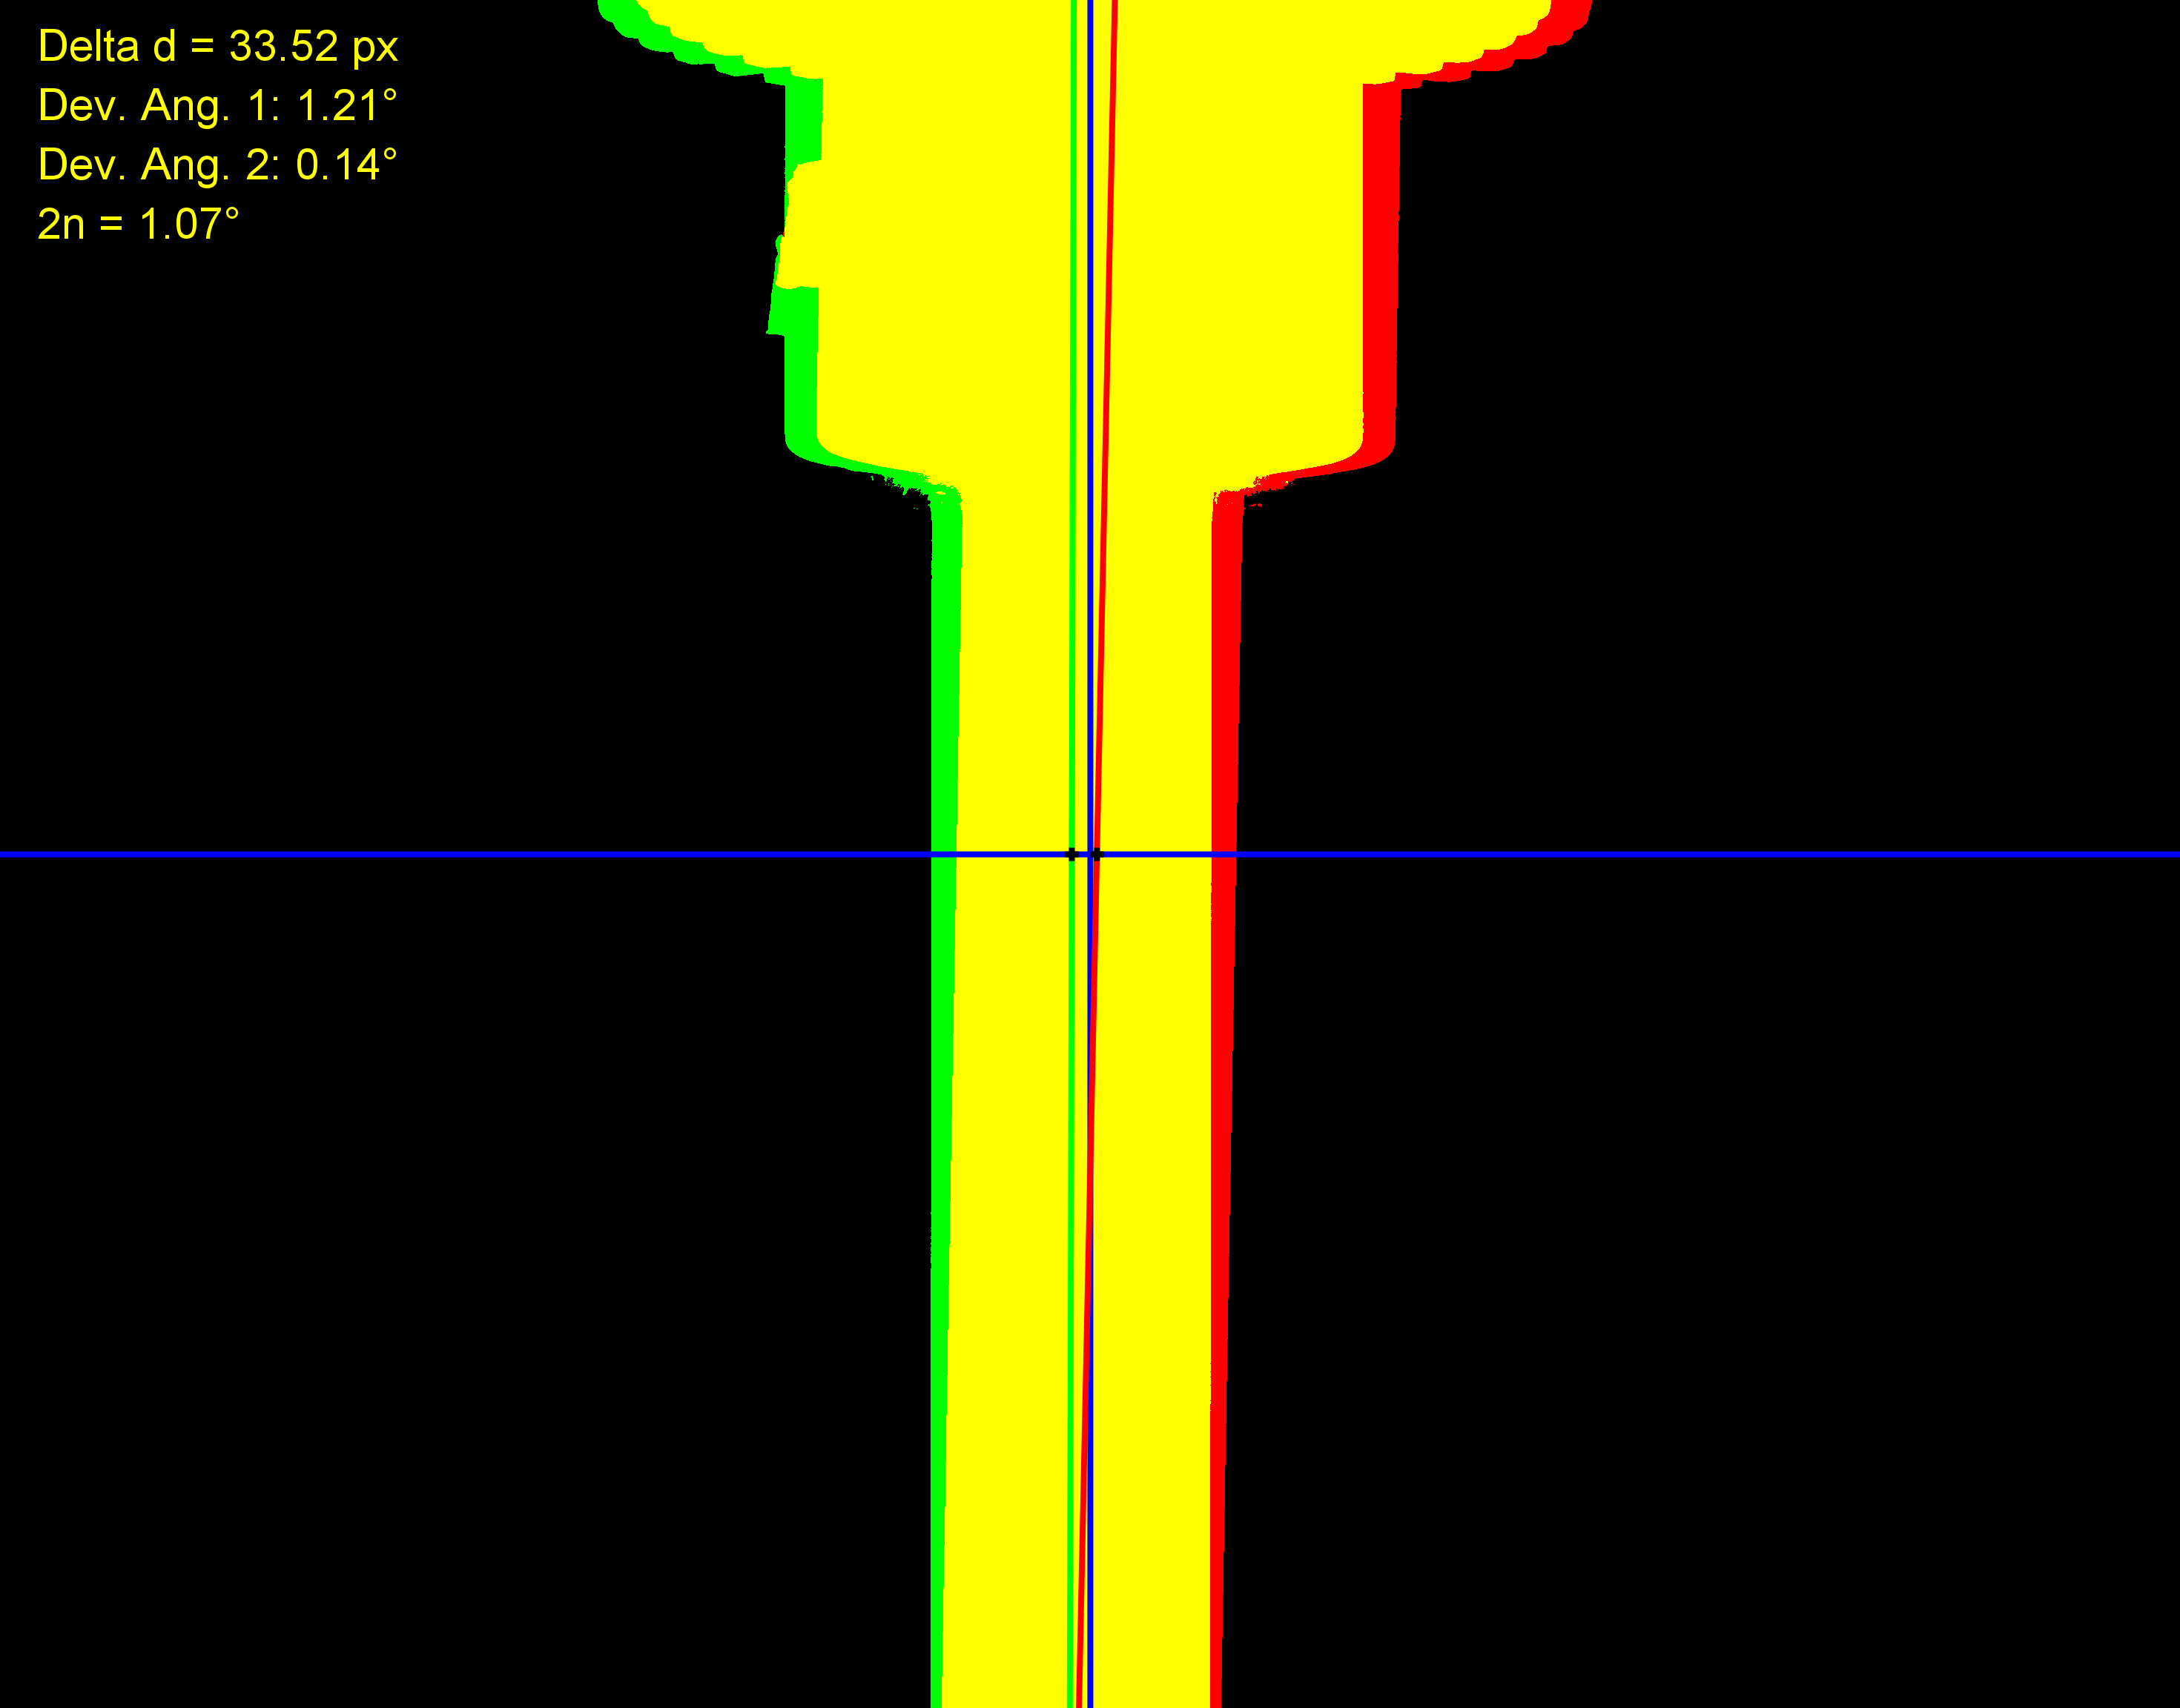
\includegraphics[width=\textwidth]{images/Interseccion_cerca.png}
    \end{subfigure}
    \hfill
    \begin{subfigure}{0.49\textwidth}
        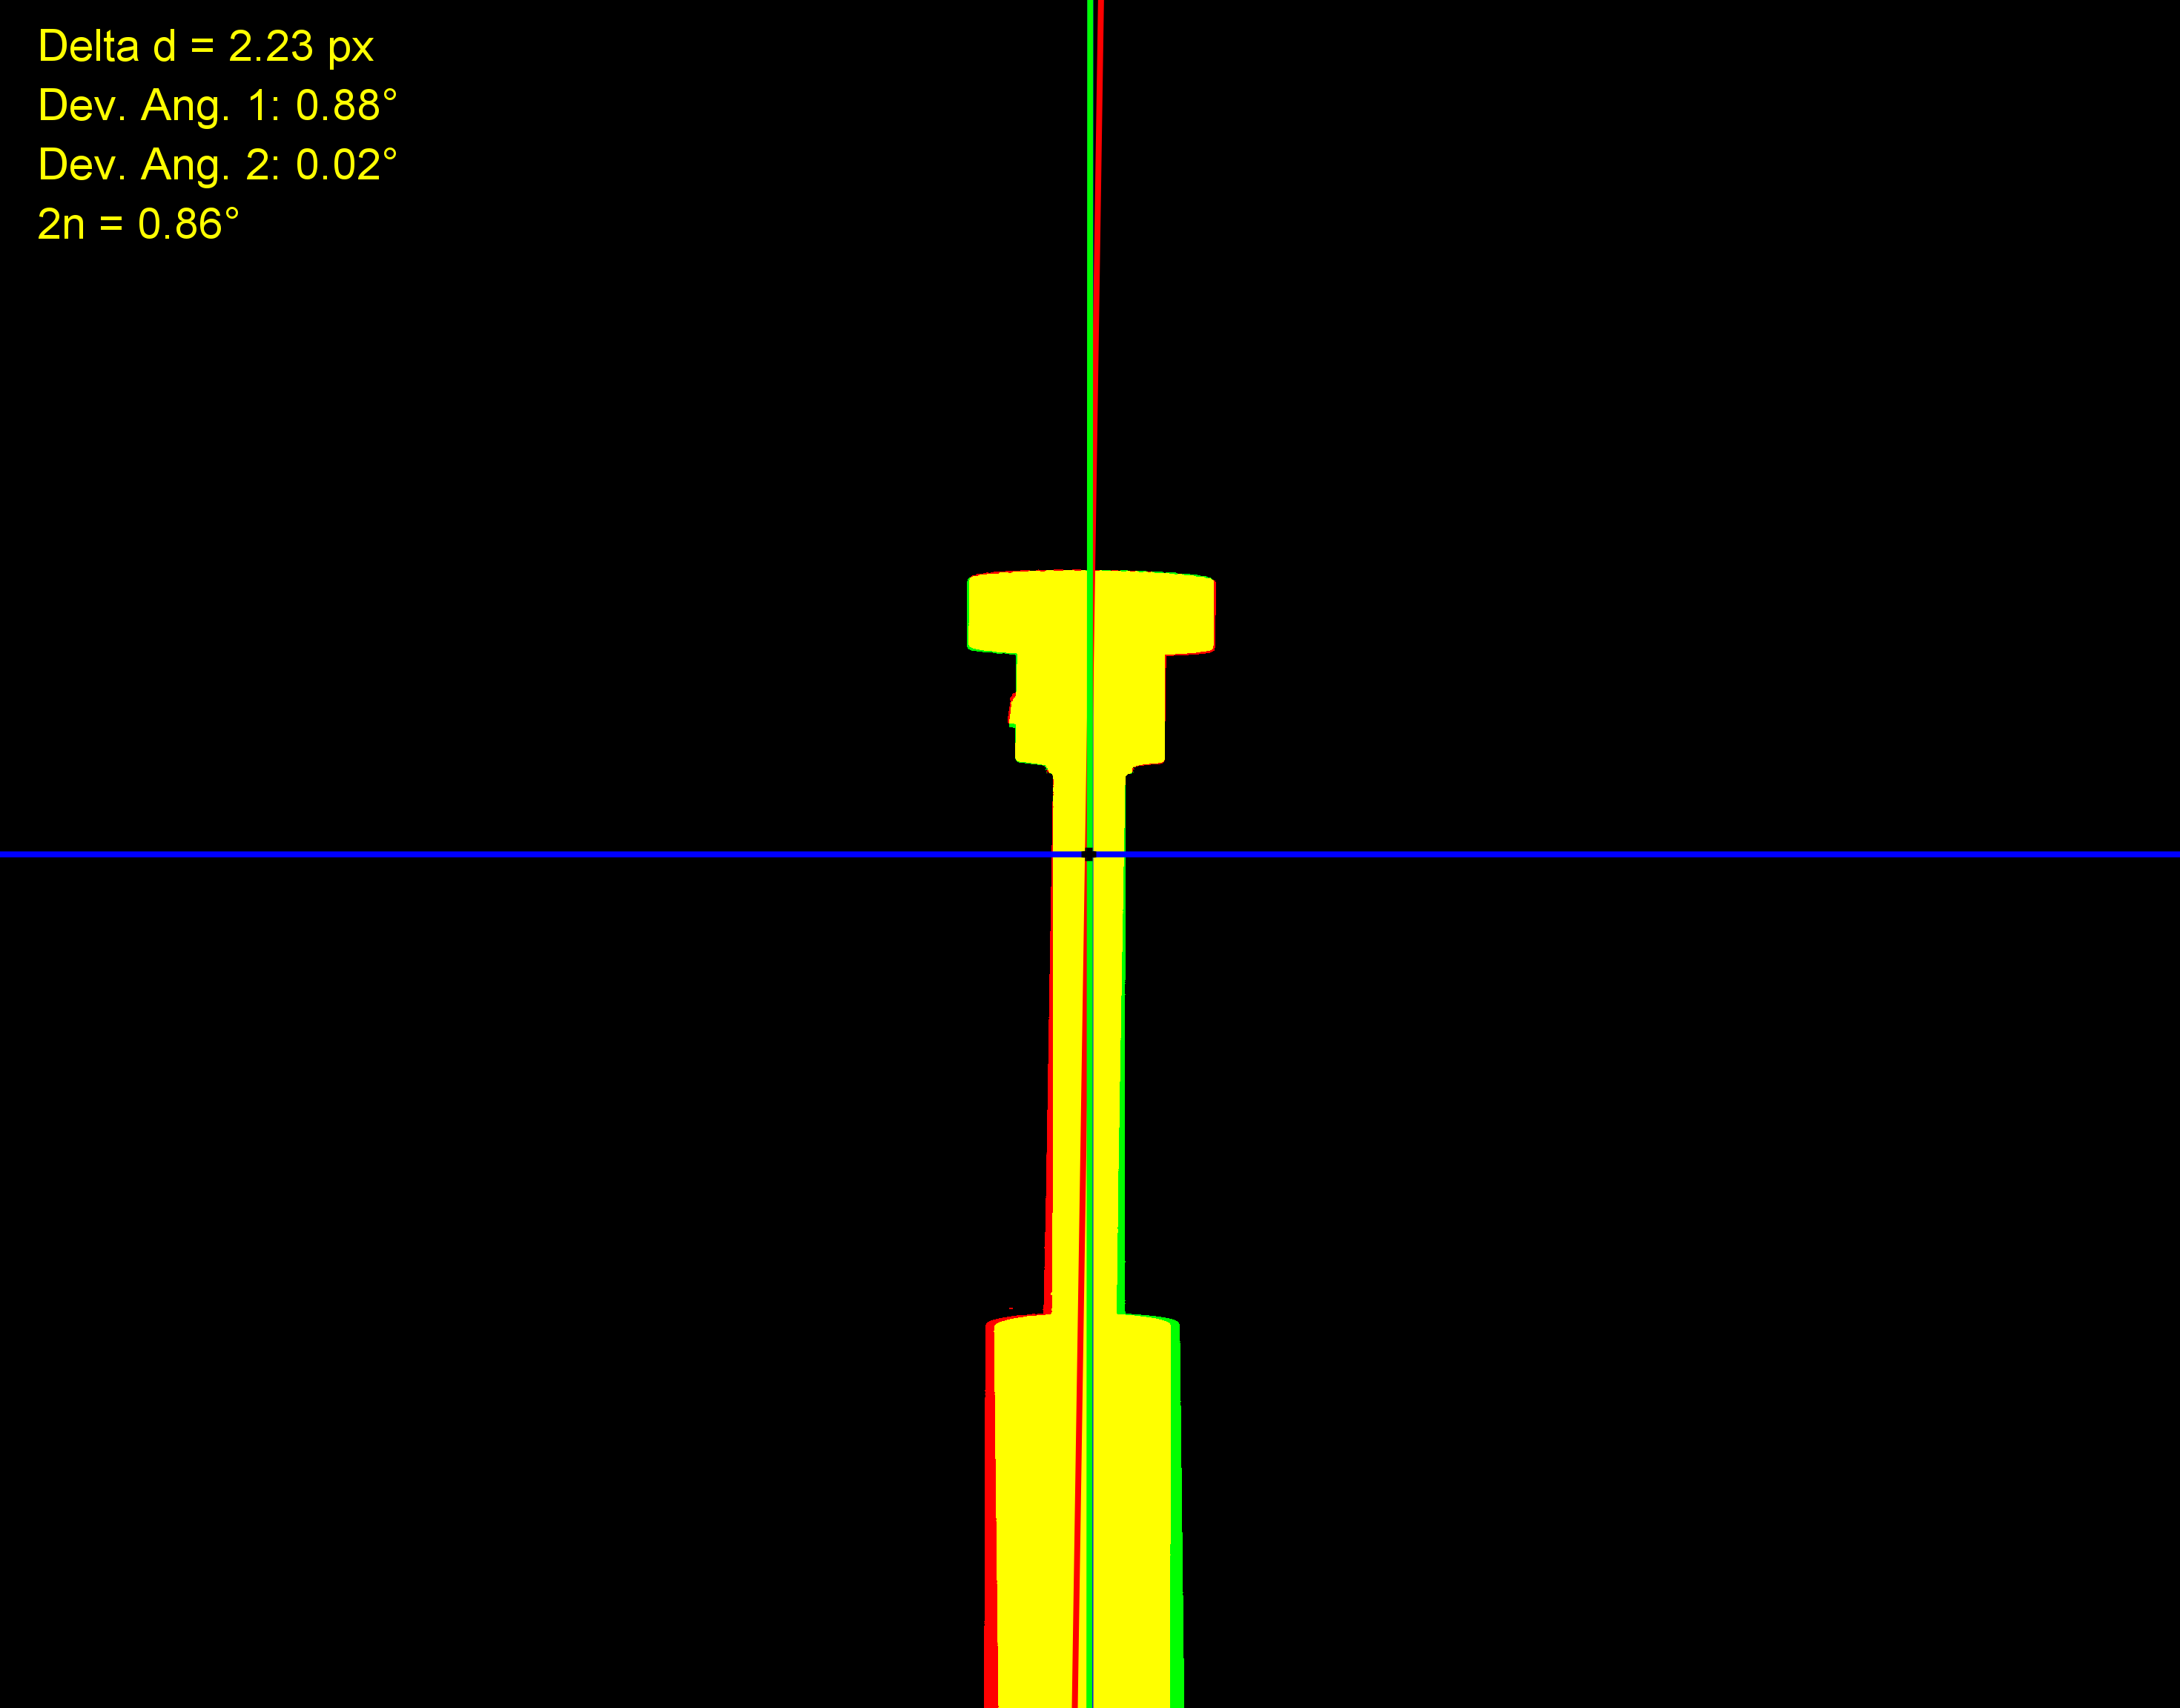
\includegraphics[width=\textwidth]{images/Interseccion_lejos.png}
    \end{subfigure}
    \caption{Cada imagen es la superposición de dos proyecciones del mismo objeto en una posición
    $\hat{x}$ (\textit{izq.} cercana a la fuente y \textit{der.} lejana). La región color verde es
    el reflejo horizontal de la proyección del objeto rotado 180$^{\circ}$ respecto de la posición original
    (rojo), y la amarilla es la superposición de ambos. Se determinan los ejes de rotación de cada
    objeto, el ángulo $2\eta$ entre ambos, y los puntos de intersección de los ejes de rotación con
    $U=0$, utilizados para determinar la distancia $\Delta d$ entre ejes.}
    \label{fig:res_alin_muestra}
\end{figure}

Los resultados anteriores son estimaciones que se obtuvieron al intentar reducir las desalineaciones
al mínimo posible, manipulando el hardware directamente. Se encuentran resumidos en la tabla
\ref{tabl:alineacion}.

Una vez realizada la alineación general, se procedió a aplicar los métodos de múltiples proyecciones
y de única proyección para
determinar las correcciones necesarias, como se explicó anteriormente. En la figura
\ref{fig:res_yang}.a se puede observar una proyección arbitraria del fantoma superpuesta
sobre un gráfico con todas las posiciones de cada una
de las esferas, a lo largo de la rotación. Por otro lado, la figura \ref{fig:res_yang}.b
muestra las elipses ajustadas a partir de las posiciones medidas, correspondientes a cada esfera,
y los puntos de interés $\vec{p}_{ij}$ ($j=0,1,2,3,4$). A partir de dichos puntos, se
realizaron los ajustes lineales necesarios (fig. \ref{fig:res_yang}.c y \ref{fig:res_yang}.d), para determinar
los valores de $\Delta U$, $\Delta V$, $\eta$ y $D$. Por último, se determinó el valor de $F$ a partir de la ecuación \ref{eq:F}, con
$l=(28.0 \pm 0.1)$ mm, la distancia entre los centros de la primera y última esfera. 

Todo el procedimiento antes explicado se realizó también al modificar el microtomógrafo y volver
a alinearlo, con las mismas distancias cercana y lejana ($D_1$ y $D_2$), y con una distancia
final (medida con instrumento) de $D = (256 \pm 1)$ mm. No se utilizó el método de una única
proyección en este caso, ya que su inconsistencia e imprecisión ya se había demostrado (ver siguiente
sección).

En la tabla \ref{tabl:alineacion}
se exponen todos los resultados de distintas mediciones con ambos métodos (junto con los valores
de $D_m$ y $F_m$ medidos con instrumentos). En particular, las mediciones marcadas con color gris
fueron realizadas tras una realineación del eje de movimiento del porta-muestra, mientras que las
color amarillo corresponden a la última modificación del microtomógrafo (con el detector en ``vertical'').
Las incertidumbres se determinaron a partir de
los ajustes finales, en el caso de los parámetros $\Delta U$, $\Delta V$, $\eta$ y $D$. Para $F$,
se tomó como incertidumbre la propagación de errores en la ecuación \ref{eq:F}, utilizando la incertidumbre
obtenida para $D$ y la estimada para $l$. Para las distancias entre puntos $\vec{p}_{ij}$, se tuvo en cuenta
que las elipses elegidas para el cálculo (la primera y la última) son las que mejor ajustan los datos,
y se observó un error geométrico menor a 0.5 px. Por otro lado,
en la tabla \ref{tabl:ajustes} se observan los valores del coeficiente de determinación $R^2$ de
todos los ajustes por regresión lineal realizados durante una medición (ocho elipses y dos rectas),
específicamente, de la cuarta medición de la tabla \ref{tabl:alineacion}, que es representativa
de todas las mediciones.


\begin{table}[htbp]
    \centering
    \caption{Parámetros de alineación y correcciones geométricas.}
    % Ajustes de reducción
    \small 
    \setlength{\tabcolsep}{4pt} % El valor por defecto es 6pt
    \begin{tabular}{ccccccc} % 7 columnas centradas
        \toprule
        \rowcolor{gray!30} \multicolumn{7}{c}{\textbf{Alineación general}} \\ \midrule
        $D$ (mm) & $\Delta \hat{Y}$ (mm) & $\theta$ ($^{\circ}$) & $\phi$ ($^{\circ}$) & $\Delta U$ (px) & $\Delta V$ (px) & $\eta$ ($^{\circ}$) \\ \midrule
        $258 \pm 1$ & $<2$ & $<4$ & $<4$ & $<5$ & $<5$ & $0.48 \pm 0.06$  \\
        \rowcolor{yellow!30} $256 \pm 1$ & $<2$ & $<4$ & $<4$ & $<9$ & $<4$ & $-0.37 \pm 0.02$  \\
        \\ \midrule % Espacio para datos

        \rowcolor{gray!30} \multicolumn{7}{c}{\textbf{Correcciones por método de múltiples proyecciones}} \\ \midrule
        $D_m$ (mm) & $F_m$ (mm) & $D$ (mm) & $F$ (mm) & $\Delta U$ (px) & $\Delta V$ (px) & $\eta$ ($^{\circ}$) \\ \midrule
        $258 \pm 1$ & $71 \pm 1$ & $268.7 \pm 0.8$ & $80.1 \pm 0.6$ & $15.0 \pm 0.9$ & $21.6 \pm 0.6$ & $0.45 \pm 0.02$ \\
        $258 \pm 1$ & $107 \pm 1$ & $266.6 \pm 0.5$ & $106.2 \pm 0.5$ & $22.4 \pm 0.7$ & $22.4 \pm 0.5$ & $0.50 \pm 0.03$ \\
        $258 \pm 1$ & $79 \pm 1$ & $267.9 \pm 0.6$ & $77.4 \pm 0.4$ & $29.6 \pm 0.7$ & $22.4 \pm 0.5$ & $0.52 \pm 0.03$ \\ \midrule
        \rowcolor{gray!15} $258 \pm 1$ & $88 \pm 1$ & $267.5 \pm 0.5$ & $87.2 \pm 0.3$ & $1.4 \pm 0.1$ & $21.6 \pm 0.5$ & $0.46 \pm 0.01$ \\
        \rowcolor{gray!15} $258 \pm 1$ & $133 \pm 1$ & $266.3 \pm 0.5$ & $132.2 \pm 0.4$ & $1.6 \pm 0.1$ & $22.6 \pm 0.5$ & $0.49 \pm 0.01$ \\ \midrule
        \rowcolor{yellow!30} $256 \pm 1$ & $93 \pm 1$ & $264.6 \pm 0.3$ & $93.1 \pm 0.4$ & $3 \pm 1$ & $-14 \pm 1$ & $-0.33 \pm 0.02$ \\
        \\ \midrule
        
        \rowcolor{gray!30} \multicolumn{7}{c}{\textbf{Correcciones por método de una proyección}} \\ \midrule
        $D_m$ (mm) & $F_m$ (mm) & $D$ (mm) & $F$ (mm) & $\Delta U$ (px) & $\Delta V$ (px) & $\eta$ ($^{\circ}$) \\ \midrule
        \rowcolor{gray!15}$258 \pm 1$ & $175 \pm 1$ & $211 \pm 2$ & $136 \pm 1$ & $-3.6 \pm 0.5$ & $11 \pm 1$ & $-39 \pm 1$ \\
        \rowcolor{gray!15}$258 \pm 1$ & $114 \pm 1$ & $264.1 \pm 0.9$ & $117 \pm 1$ & $0.5 \pm 0.9$ & $1.1 \pm 0.5$ & $2.3 \pm 0.7$ \\
        \rowcolor{gray!15}$258 \pm 1$ & $220 \pm 1$ & $264 \pm 1$ & $225 \pm 1$ & $-2 \pm 1$ & $-5 \pm 1$ & $-17 \pm 2$ \\
        \rowcolor{gray!15}$258 \pm 1$ & $220 \pm 1$ & $265 \pm 1$ & $226 \pm 1$ & $-13 \pm 2$ & $10 \pm 2$ & $48 \pm 4$ \\
        \bottomrule
    \end{tabular}
\label{tabl:alineacion}
\end{table}

\begin{table}[htbp]
\centering
\caption{Coeficientes de determinación de ajustes, para método de Yang.}
\begin{tabular}{cccccccccc}
    \toprule
    \rowcolor{gray!30} \multicolumn{10}{c}{\textbf{Coeficiente de determinación $R^2$}} \\ \midrule
    Esf 1 & Esf 2 & Esf 3 & Esf 4 & Esf 5 & Esf 6 & Esf 7 & Esf 8 & $\{ D, \Delta V \}$ & $\{\eta, \Delta U \}$ \\ \midrule
    \rowcolor{gray!15} $0.997$ & $0.995$ & $0.985$ & $0.891$ & $0.857$ & $0.996$ & $0.999$ & $0.999$ & $0.999$ & $0.998$ \\
    \rowcolor{yellow!30} $0.998$ & $0.996$ & $0.988$ & $0.864$ & $0.958$ & $0.998$ & $0.999$ & $0.999$ & $0.999$ & $0.980$ \\ \bottomrule
\end{tabular}
\label{tabl:ajustes}
\end{table}

\begin{figure}[htbp] % Se recomienda htbp en lugar de h para dar más opciones de posicionamiento al compilador
    \centering
    % Primera fila
    \begin{overpic}[width=0.49\linewidth]{images/plot_centroids2.png}
        \put(2, 75){\colorbox{black!50}{\color{white}\bfseries\large (a)}}
    \end{overpic}\hfill
    \begin{overpic}[width=0.49\linewidth]{images/fit_elipses.png}
        \put(2, 75){\colorbox{black!50}{\color{white}\bfseries\large (b)}}
    \end{overpic}
    
    \vspace{2ex} % Espaciado entre filas
    
    % Segunda fila
    \begin{overpic}[width=0.49\linewidth]{images/yang_fit_1.png}
        \put(2, 75){\colorbox{black!50}{\color{white}\bfseries\large (c)}}
    \end{overpic}\hfill
    \begin{overpic}[width=0.49\linewidth]{images/yang_fit_2.png}
        \put(2, 75){\colorbox{black!50}{\color{white}\bfseries\large (d)}}
    \end{overpic}
    
    \caption{\textbf{a)} Una proyección arbitraria del fantoma, puesta sobre un gráfico que
    contiene las posiciones de todos los centros de las esferas, a lo largo de toda su trayectoria
    en 360$^{\circ}$. \textbf{b)} Elipses ajustadas a partir de las posiciones medidas, con los puntos de interés $\vec{p}_{ij}$ marcados (centros y vértices).
    \textbf{c)} Ajuste lineal de los puntos $(x_i,y_i)$ definidos en la ecuación
    \ref{eq:variables_yang1}. A partir de los parámetros $\mathsf{a}_1$ y $\mathsf{b}_1$
    se pueden obtener los valores de $D$ y $\Delta V$. \textbf{d)} Ajuste lineal de los
    puntos $(v_{i0},u_{i0})$; a partir de los parámetros $\mathsf{a}_2$ y $\mathsf{b}_2$
    se pueden calcular $\Delta U$ y $\eta$.}
    \label{fig:res_yang}
\end{figure}

\section{Resolución espacial}

\subsection{Análisis por MTF}

Uno de los objetivos de la calibración geométrica, es poder determinar con precisión
la resolución espacial de una tomografía/radiografía, ya que de esta dependen todas las
mediciones de distancias que se quieran realizar. La ecuación \ref{eq:res_espacial},
aunque más completa que solo considerar la magnificación de un objeto por una fuente
puntual, sigue siendo una aproximación, ya que la resolución depende de todos los elementos
del sistema (fuente, objeto, detector, electrónica, algoritmos, etc.). Sin embargo,
esta se puede medir directamente en una radiografía.

El método más directo consiste en utilizar un objeto de referencia, con detalles de
tamaño similar a la resolución (por ejemplo, líneas y círculos). El problema es que,
para microtomógrafos con resolución en el orden de micrómetros, es difícil producir
fantomas apropiados. El método más común es el análisis de bordes por medio de la
función de transferencia de modulación (\textit{Modulation Transfer Function} - $MTF$)\cite{Buzug2008}.
La $MTF$ es una función que relaciona la frecuencia espacial a la correspondiente
pérdida de contraste en la imagen, y se define como la transformada de Fourier de la
derivada de la función de dispersión de borde (\textit{Edge Spread Function} - $ESF$), y se define normalizada. La $ESF$ es la función de
contraste o intensidad $I(x)$, en la dirección $x$ que atraviesa perpendicularmente una interfaz o borde,
y su derivada se conoce como la función de transferencia de línea (\textit{Line Transfer
Function} - $LSF$). \cite{Samei1998}\cite{Rueckel2014}

\begin{equation}
    MTF(k_x) = \dfrac{\mathcal{F}\left\{LSF(x)\right\}}{MTF(0)} =
    \dfrac{\mathcal{F}\left\{\dfrac{d}{dx}ESF(x)\right\}}{MTF(0)}
    \label{eq:MTF}
\end{equation}

\noindent donde $\mathcal{F}\left\{f(x)\right\}(k_x)$ es la Transformada de Fourier de la
función $f(x)$, del dominio espacial $x$ al dominio de frecuencias $k_x$.

A medida que aumenta la frecuencia espacial $k_x$ en la dirección $x$, mayor es la pérdida
de constraste, es decir, mientras más cercanos sean dos detalles distintos (líneas o puntos),
más difícil es diferenciarlos en la imagen. Para obtener un valor específico de la
resolución espacial, en general se considera la frecuencia espacial $k_c$ a la que la
función $MTF$ cae al 10$\%$ \cite{Ruf2020}, de la que puede obtenerse el valor correspondiente en el
dominio espacial mediante la ecuación \ref{eq:res_espacial}.

A partir de esto, se midió la $MTF$ de dos formas. En la primera, se utilizó como fantoma
una lámina metálica, de ancho $w_{lamina}= (12.56\pm 0.02)$ mm y borde recto, fijada por un marco de acrílico de
tal forma que hay una sección de solo aire y metal (ver figura \ref{fig:chapita}.a). El fantoma se coloca en el porta-muestra,
idealmente perpendicular al eje del haz, y se obtienen proyecciones a distintas
magnificaciones $M$. El borde de la lámina debe estar inclinado con respecto a los ejes
$(u,v)$, para evitar posibles distorsiones por filas/columnas de pixeles en el detector.
El borde es rotado en el procesamiento de la imagen, para alinearlo nuevamente, y se mide
el perfil de contraste entre el aire y la lámina (en una dirección perpendicular al borde).
En concreto, se mide el valor medio de cada columna $x$, $VM|_{y_0}^{y_f}(x)$, en un ROI alrededor del borde.
Posteriormente, se interpola la función $ESF(x)$ a partir de los puntos obtenidos,
y se calcula la derivada numérica. Finalmente, se realiza una transformada de Fourier rápida (FFT) y,
normalizando con el valor correspondiente a $k_x = 0$, se obtiene la $MTF(k_x)$. Para obtener
un valor más representativo de todo el borde, se realizan múltiples mediciones en distintos
ROIs a lo largo del borde (utilizando un \textit{macro} en FIJI, ver Apéndice B.4), como se observa en la figura
\ref{fig:chapita}.b.

\begin{figure}[htpb]
    \centering
    \begin{subfigure}{0.35\textwidth}
        \begin{overpic}[width=\linewidth]{images/phantom_chapita.jpg}
            \put(2, 87){\colorbox{black!60}{\color{white}\bfseries\large (a)}}
        \end{overpic}
    \end{subfigure}
    \hspace{5mm}
    \begin{subfigure}{0.45\textwidth}
        \begin{overpic}[width=\linewidth]{images/chapita_esf.png}
            \put(2, 68){\colorbox{black!60}{\color{white}\bfseries\large (b)}}
        \end{overpic}
    \end{subfigure}
    \caption{\textbf{a)} Fantoma utilizado para medir resolución espacial de una
    proyección. Lámina delgada de metal, en contacto con aire y ligeramente inclinada
    con respecto a los ejes del detector. \textbf{b)} Proyección del fantoma. Los
    rectángulos rojos son los ROIs sobre los que se analiza el perfil de intensidad, en
    la dirección del lado largo.}
    \label{fig:chapita}    
\end{figure}

Para la interpolación de $ESF(x)$, se realiza un ajuste polinómico móvil de orden 4 con peso gaussiano,
es decir, se ajusta un polinomio de orden 4 a los datos dentro de una ``ventana'' de
ancho $w_v$, la cual se va desplazando por todo el set. A partir de los coeficientes
obtenidos en cada ventana, es posible interpolar los puntos cercanos a cada dato. 
Para un polinomio de orden 4, $w_v$ debe contener al menos cuatro puntos consecutivos
(cinco si se cuenta el punto central), y mientras más grande es, produce un mayor
suavizado de la función (lo cual puede afectar el resultado del $MTF$) \cite{Samei1998}.
Para este trabajo, se utilizó $w_v = 5$ y una interpolación de factor 2 (se duplica
la cantidad de datos). Por otro lado, para obtener una medición más ``limpia'' del $MTF$
se recomienda aplicar un filtro de Hamming a la $LSF$, con tal de eliminar los componentes
de frecuencias altas.

Sin embargo, este método determina la resolución espacial de una radiografía, y aunque
la intuición indica que esta debería ser la misma que una tomografía, esta podría ser
alterada por algún efecto de la reconstrucción. Luego, se realizó el siguiente método para
medir la resolución espacial de una tomografía, basado en la investigación de Ruf \textit{et al.}
\cite{Ruf2020}. La idea es obtener una reconstrucción de un fantoma cilíndrico, y aplicar
el mismo procedimiento que con la lámina, pero analizando distintas slices (cortes 
transversales) o cortes sagitales a lo largo del diámetro completo (ver fig. 
\ref{fig:fantoma_MTF}). Así, se pueden obtener mediciones de la resolución espacial de 
la tomografía, en distintas direcciones de reconstrucción. Para obtener dichos cortes,
se utilizó un \textit{macro} (ver Apéndice B.5).

\begin{figure}[htbp]
    \centering
    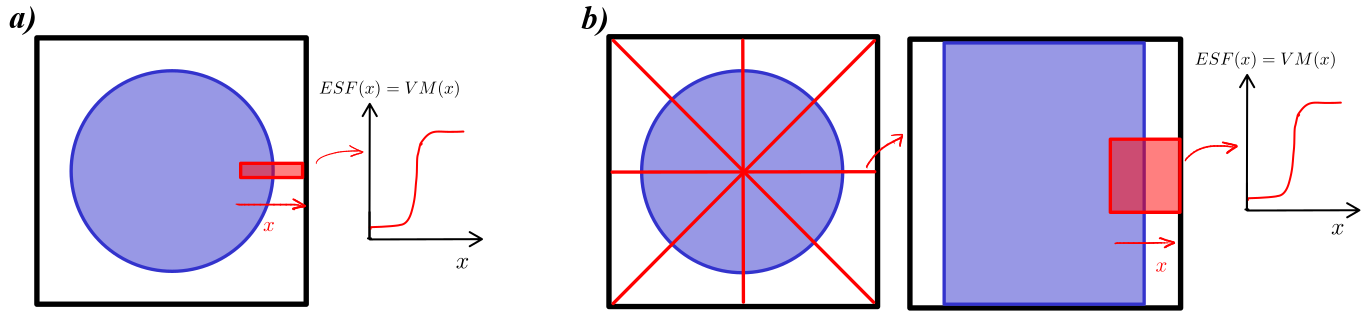
\includegraphics[width=\textwidth]{images/fantoma_MTF.png}
    \caption{Proceso de medición del $ESF(x)$ en una reconstrucción tomográfica de un
    cilindro. \textbf{a)} Adquisición de $ESF(x)$ en un corte axial, seleccionando una
    región alrededor del borde, con la menor curvatura posible. \textbf{b)} Adquisición
    de $ESF(x)$ en un plano sagital, seleccionando una región alrededor del borde.}
    \label{fig:fantoma_MTF}
\end{figure}

\subsection{Resultados}

En la figura \ref{fig:res_mtf_1} pueden observarse tres gráficos (a, b y c) representativos de
todo el proceso (utilizando la lámina): la adquisición e interpolación de la $ESF(x)$, la derivada o $LSF(x)$
y la obtención de la $MTF(k_x)$, para una magnificación específica. La figura \ref{fig:res_mtf_1}.d
muestra las mediciones obtenidas de la resolución espacial a partir de este método, para
distintas magnificaciones, en cada uno de los sistemas alineados (rojo, sistema inicial con
detector horizontal; azul, sistema final con detector vertical), y las compara con las curvas correspondientes a la ecuación
\ref{eq:res_espacial} (para tamaños focales $s_1 = 0.005$ mm y $s_2 = 0.007$ mm, correspondientes a
la fuente utilizada). Los valores de resolución
espacial se calcularon como $RE = 1/(2k_c)$, donde $k_c$ es la frecuencia de corte ($MTF(k_c)=0.1$).
La incertidumbre se calculó propagando la incertidumbre de $k_c$, la cual fue definida como
el error estadístico a partir de 10 mediciones de $MTF$ a lo largo del borde.

También, a partir de las mediciones de resolución espacial en conjunto, se realizó un ajuste de los
datos a la siguiente curva, basada en la ecuación \ref{eq:res_espacial}, pero agregando un parámetro
extra $c$ que contribuye al tamaño de pixel $\Delta p$, y con $S=s_2$. El mismo se encuentra
graficado en la figura \ref{fig:res_mtf_1}.d, y tiene un coeficiente de determinación $R^2 = 0.983$ y
un valor del parámetro ajustado $c=(0.0264 \pm 0.0008)$ mm.

\begin{equation}
    RE(M) = \sqrt{\left(S\cdot\dfrac{M-1}{M}\right)^2 + \left(\dfrac{\Delta p+c}{M}\right)^2}
    \label{eq:ajuste_resolucion}
\end{equation}

Por otro lado, para el análisis de la resolución espacial de una tomografía, se utilizó una
reconstrucción de un cilindro con una magnificación $M\sim 5.2$. Se analizó el perfil
de intensidad de borde en 10 re-proyecciones radiales. Los gráficos de $ESF(x)$, $LSF(x)$
y $MTF(x)$ pueden observarse en la figura \ref{fig:res_mtf_2}. Promediando los valores
de frecuencia de corte se obtiene que, para esta magnificación, $k_c = (28.5 \pm 0.3)$ lp/mm,
y la resolución espacial, $RE = (17.5 \pm 0.2)$ $\mu$m, valor que se agregó al gráfico de la
figura \ref{fig:res_mtf_1}.d.

\begin{figure}[htbp]
    \centering
    % Primera fila
    \begin{overpic}[width=0.49\linewidth]{images/ESF.png}
        \put(2, 75){\colorbox{black!50}{\color{white}\bfseries\large (a)}}
    \end{overpic}\hfill
    \begin{overpic}[width=0.49\linewidth]{images/LSF.png}
        \put(2, 75){\colorbox{black!50}{\color{white}\bfseries\large (b)}}
    \end{overpic}
    
    \vspace{2ex} % Espaciado entre filas
    
    % Segunda fila
    \begin{overpic}[width=0.49\linewidth]{images/MTF_1.png}
        \put(2, 75){\colorbox{black!50}{\color{white}\bfseries\large (c)}}
    \end{overpic}\hfill
    \begin{overpic}[width=0.49\linewidth]{images/resolucion.png}
        \put(2, 75){\colorbox{black!50}{\color{white}\bfseries\large (d)}}
    \end{overpic}
    
    \caption{\textbf{a)} Función $ESF(x)$ ajustada al perfil de intensidad de un
    ROI alrededor de un borde. \textbf{b)} Función $LSF(x)$, derivada numérica de $ESF(x)$.
    \textbf{c)} Función $MTF(k_x)$, la transformada de Fourier de $LSF(x)$ y normalizada. El
    valor de $k_x$ para el que $MTF=0.1$ se denomina \textit{frecuencia de corte} $k_c$,
    y es considerada como la resolución espacial del sistema. \textbf{d)} Mediciones de
    $RE$ en función de la magnificación $M$, a partir de un promedio de 10 mediciones de
    $MTF$ cada una, de las dos configuraciones del sistema (rojo para el detector horizontal;
    azul para el detector vertical); también se grafican las curvas de resolución mínima ideal (para tamaños
    de foco $s_1$ y $s_2$), y la curva de ajuste a los datos en conjunto (ecuación \ref{eq:ajuste_resolucion}),
    y la medición de $RE$ obtenida a partir de una reconstrucción tomográfica.}
    \label{fig:res_mtf_1}
\end{figure}

\begin{figure}[htbp]
    \centering
    \begin{subfigure}{0.32\textwidth}
        \begin{overpic}[width=\linewidth]{images/ESF_tomgr.png}
            \put(2, 75){\colorbox{black!50}{\color{white}\bfseries\large (a)}}
        \end{overpic}        
    \end{subfigure}
    \hfill
    \begin{subfigure}{0.32\textwidth}
        \begin{overpic}[width=\linewidth]{images/LSF_tomgr.png}
            \put(2, 75){\colorbox{black!50}{\color{white}\bfseries\large (b)}}
        \end{overpic}        
    \end{subfigure}
    \hfill
    \begin{subfigure}{0.32\textwidth}
        \begin{overpic}[width=\linewidth]{images/MTF_2.png}
            \put(2, 75){\colorbox{black!50}{\color{white}\bfseries\large (c)}}
        \end{overpic}        
    \end{subfigure}
    \caption{\textbf{a)} $ESF(x)$ de distintos cortes radiales de la reconstrucción tomográfica
    de un cilindro metálico. \textbf{b)} $LSF(x)$ de los distintos cortes. \textbf{c)}
    $MTF(k_x)$ de los distintos cortes reconstruidos, y $MTF_{promedio}$.}
    \label{fig:res_mtf_2}
\end{figure}

\section{Discusiones}

\subsection{Alineación y correcciones}

Observando los resultados de la tabla \ref{tabl:alineacion}, se puede ver que una buena alineación
general es posible de lograr, utilizando los métodos de análisis de círculos proyectados y
superposición de cilindros rotados. La figura \ref{fig:alineacion_fuente} muestra que los círculos
proyectados alcanzan criterios de circularidad satisfactorios, con $C_W \sim 90\%$ y $R \sim 99\%$.
La razón por la que $C_W$ no es mayor, se debe a que el cálculo de perímetro y área se realiza
contando píxeles en una grilla discreta, lo que produce un error geométrico al tratarse de una
figura curva. La importancia de estos resultados radica en la capacidad de alinear la orientación
del detector, con respecto a la fuente, llegando a lograr una desviación angular menor a 5$^{\circ}$ respecto
de la posición ideal, solamente observando una proyección.

Sin embargo, este proceso depende mucho de la destreza
del operador, por lo que es difícil de estandarizar. Otro problema relacionado con esto, es que
se asume que al mover el detector a su posición final, se hace a lo largo de un eje que une
las posiciones cercana y lejana. Sin embargo, este traslado está lejos de ser ideal, debido al
juego mecánico de la base sobre la que se mueve, los tornillos de ajuste, la fricción, etc. Este
problema puede solucionarse mejorando el sistema de la base, utilizando mejores piezas y rieles,
y en última instancia, con un sistema de movimiento motorizado, que asegure un traslado suave
y consistente. Por esta razón es que se observan diferencias entre los parámetros $\Delta U$ y $\Delta V$ obtenidos
con los métodos de proyecciones, con respecto a los valores esperados a partir de la alineación general.

Una utilidad de este método, es la posibilidad de estimar los ángulos $\theta$ y $\phi$, o más bien,
demostrar que estos son lo suficientemente pequeños como para aplicar el método de múltiples proyecciones
posteriormente. Esto se mantiene en la posición final, utilizando escuadras y niveles. Sin
embargo, no es posible medirlos con mayor precisión, debido a no poder estudiar el círculo
proyecado.

Sobre el análisis de la superposición de cilindros rotados, se observa en la tabla que los resultados
estimados de $\eta$ son comparables a los obtenidos con el método de múltiples proyecciones, por lo que es
viable como un método más rápido para determinar este parámetro. Sin embargo, se presenta otro
problema, difícil de contemplar en el análisis: el método asume que el cilindro está perfectamente
alineado con el eje de rotación del porta-muestra (esta asunción se hace con cualquier muestra en realidad),
sin embargo, después de estudiar numerosas veces este proceso, se observa que esto varía según el
tamaño y forma del objeto, y la forma en que se lo fija al porta-muestra. Así, se tiene que el
valor obtenido de $\eta$, a pesar de ser la inclinación del eje de rotación y ser consistente, no
necesariamente es el ángulo de inclinación del objeto, sino una aproximación a primer orden de este.
Este problema es difícil de solucionar por corrección de software, ya que dicha inclinación
varía según el objeto y no siempre es posible medirla con precisión. La solución más viable es
mejorar los sistemas de fijación de la muestra y/o bases utilizadas en el porta-muestra.
Este problema se presenta sobre todo, en muestras de gran tamaño o forma muy irregular, aunque en
muestras pequeñas no es tan prevalente.

A la hora de analizar y comparar los métodos de corrección, se tienen en cuenta tres criterios:
preparación, adquisición y resultados, siendo este último el más importante. En cuanto a la preparación
y adquisición, el método de una única proyección parece ser el más rápido y sencillo, ya que en principio
se necesita una sola radiografía del fantoma, de ahí lo atractivo del método. Y aunque es cierto
que el método de múltiples proyecciones tiene un tiempo de adquisición mucho mayor (se tardó alrededor de
20 minutos en obtener las 360 proyecciones), la preparación es relativamente sencilla comparada al otro.
En particular, el de una única proyección tiene una serie de condiciones más exigentes para su aplicación,
algunas de las cuales son prácticamente equivalentes a las condiciones de alineación general del sistema.

En primer lugar, como se mencionó en el procedimiento, el método de ``una única proyección'' requiere en realidad
más de una proyección para poder asegurar una orientación del cuadrado perpendicular con el eje
$\mathcal{M}$. Pero principalmente, este método requiere que el eje de magnificación pase justo por el centro del cuadrado. Esto
es imposible de determinar a partir de la proyección del fantoma, ya que se asume que el detector y la
fuente están desalineados (en efecto, se desea determinar $\Delta U$ y $\Delta V$), por lo que dicha
apreciación se debe realizar observando el sistema directamente. Esto es especialmente difícil cuando
el fantoma se encuentra medianamente alejado de la fuente. Quizá con mejores instrumentos de medición,
sería posible cumplir esta condición, pero a este punto la preparación del método requeriría tanto o más
esfuerzo que la alineación en sí. Además, el método es muy sensible a esta condición, como se observa en
los resultados obtenidos en la tabla \ref{tabl:alineacion}, donde las últimas dos filas de la sección de
una única proyección se corresponden a una misma distancia $F$ pero con una variación en altura del fantoma,
menor a 1.5 mm. Los resultados obtenidos para $D$ y $F$ son comparables, ya que estos dependen principalmente
de las longitudes magnificadas de los lados (que práctimante no cambian por una variación de altura tan pequeña),
pero los valores de $\Delta U$, $\Delta V$ y $\eta$ son completamente distintos. Al ser tan sensible a esta
condición, el método se vuelve inconsistente e impráctico.

Mientras tanto, el método de múltiples proyecciones requiere solamente que el cilindro esté lo suficientemente
alineado con el eje de rotación, pero no exige una altura específica, solo que el eje de magnificación
pase entre la primera y última esfera. Esto último sí puede determinarse con facilidad a partir
de la proyección, observando la excentricidad de las elipses obtenidas (mientras más excentrica una elipse
más cerca está a la altura por la que pasa el eje $\mathcal{M}$, ver figura \ref{fig:res_yang}.b).

En cuanto a los resultados, el método de múltiples proyecciones es claramente superior, ya que presenta
resultados consistentes y precisos. En la tabla \ref{tabl:alineacion} se observa que los valores obtenidos
para los distintos parámetros son comparables entre sí, a pesar de ser mediciones tomadas en distintas
distancias $F$. Solamente las primeras 3 entradas de la tabla (con fondo blanco), presentan mayor
variación en los valores de $F$, $\Delta U$ y $\eta$. Justamente a partir de la gran variación de $\Delta U$
(y no de $\Delta V$), se determinó que se debía realizar una mejor alineación del eje de movimiento
del porta-muestra. Posterior a esto, las mediciones (con fondo gris) son mucho más consistentes entre
sí en todos los parámetros, sin importar $F$. Al contrario, el método de una única proyección presenta
resultados inconsistentes entre sí, y con mucho mayor diferencia respecto a valores esperados de
la alineación general y las mediciones realizadas con instrumentos. Esto se debe, no solo a las condiciones
estrictas que se mencionaron anteriormente, sino al hecho de que los parámetros se obtienen después de
una larga cadena de operaciones matemáticas, algunas basadas en ecuaciones no lineales y sin solución
analítica, como se observa en el Apéndice A, partiendo de pocos datos (tan solo las longitudes magnificadas medidas). De esta forma, cualquier
error en la medición inicial se ve amplificado a lo largo de todo el proceso, resultando en valores tan
distintos incluso con condiciones iniciales similares.

También es importante destacar un resultado que se observa
en todas las instancias de este método, que es la diferencia entre los valores de $D_m$ (distancia
fuente-detector medida con instrumento) y $D$ obtenida a partir de los ajustes. Esta diferencia
es aproximadamente la misma en todas las mediciones (incluso al modificar el microtomógrafo), y es
un valor promedio de 9.3 mm, lo que indicaría un error sistemático en la medición de $D_m$. Esto
podría deberse a alguna característica propia del detector, de tal forma que el área donde se
produce efectivamente la detección de los fotones se encuentre alrededor de 9 mm adentro. Se
desconoce su causa ya que no se menciona nada al respecto en el manual, pero esto se corrobora
al estudiar la magnificación de un objeto de dimensiones conocidas (como el cilindro) o analizando
los círculos proyectados del cono (ver figura \ref{fig:res_alin_fuente}). En concreto, sabiendo que
el semi-ángulo de apertura del cono es 19.5$^{\circ}$, y midiendo el radio de los círculos proyectados,
se puede determinar la distancia $D$ sabiendo que $D = r/\tan(19.5\text{$^{\circ}$})$. Para los radios obtenidos
en la figura \ref{fig:res_alin_fuente}, por ejemplo, se estiman valores de $D$ mayores a los esperados
($D_1$ y $D_2$), por más de 10 mm.

Los ajustes realizados para el método de múltiples proyecciones presentan coeficientes de determinación
$R^2$ muy cercanos a 1, como se observa en la tabla \ref{tabl:ajustes}. En el caso de los ajustes de
elipses, este valor es menor para las esferas centrales, lo que se debe a una mayor excentricidad de
las mismas al estar tan cerca del eje de magnificación. Esto también se observa en la figura \ref{fig:res_yang}.d,
donde los puntos correspondientes a las esferas centrales son los que más se apartan de la recta (ya que
son determinados a partir de los ajustes de las elipses). Sin embargo, para el resto de elipses se tiene
un $R^2>0.98$, al igual que las rectas obtenidas en los ajustes posteriores, por lo que se puede concluir
que el método de múltiples proyecciones es un método confiable para determinar los parámetros de alineación
y corrección. La mayor limitación que se encontró con este método, es el hecho de que el fantoma utilizado
funciona mejor en un rango limitado de distancias, debido a la cantidad de esferas y su distribución. Sin
embargo, esto se puede solucionar fácilmente diseñando uno nuevo, con más esferas, que pueda emplearse
en distancias más lejanas a la fuente.

\subsection{Resolución espacial}

Observando la figura \ref{fig:res_mtf_1}.d, se puede ver con claridad que la ecuación \ref{eq:res_espacial}
subestima la resolución espacial ``efectiva'' del sistema. Esta diferencia se debe a otros efectos
propios de la transferencia de la señal, que no se tienen en cuenta. Así, se tiene que este
microtomógrafo tiene una resolución espacial real de entre 15 y 60 $\mu$m (en el rango de distancias que
es utilizable).

También se observa que los resultados son comparables entre las dos configuraciones del sistema, lo
que da indicios de la consistencia de los métodos de alineación y corrección utilizados hasta ahora.
De hecho, considerando todos estos datos en conjunto, es que se realizó el ajuste de la ecuación
\ref{eq:ajuste_resolucion}, como una corrección a la ecuación \ref{eq:res_espacial}. La curva obtenida,
que predice muy bien los datos, es solamente una parametrización del sistema. Es decir, el término añadido
$c$ no tiene un significado físico específico, sino que se agregó como una corrección a la
primera ecuación, para poder describir mejor el comportamiento del microtomógrafo sobre el que se
trabajó. Aún así, observando los resultados podría interpretarse que el sistema es equivalente a uno
ideal (es decir, que solo considera al tamaño de pixel, tamaño focal y la magnificación como únicos
factores influyentes) con tamaño de foco $S=0.007$ mm y tamaño de pixel $\Delta p' = \Delta p + c = 0.0759$ mm, mayor al real.

Por último, se observa que la resolución espacial obtenida a partir de la reconstrucción tomográfica
del cilindro, es similar a la obtenida por la proyección de la lámina. Ciertamente, los pasos intermedios
presentan diferencias con respecto al método de la lámina, gracias al efecto que produce el endurecimiento
del haz en la función $ESF(x)$, lo cual afecta posteriormente a las curvas $LSF(x)$ y $MTF(k_x)$.
Sin embargo, el resultado final no dista demasiado de lo esperado a partir de la curva empírica obtenida.
El valor obtenido de $RE$
a partir de la curva ajustada para $M=5.2$ es de 15.7 $\mu$m, mientras que el valor medido directamente fue
(17.5 $\pm$ 0.2) $\mu$m (punto negro en la figura \ref{fig:res_mtf_1}). La curva parece subestimar ligeramente el valor, pero en general se puede
considerar que ambos métodos son prácticamente equivalentes para medir la resolución espacial. Esto
es ideal, ya que el método de la lámina es mucho más sencillo y rápido de implementar, y no requiere
realizar una reconstrucción tomográfica. 